
\documentclass[journal]{IEEEtran}

\usepackage{graphicx}

\graphicspath{{imfigures/}}

\usepackage{subcaption}

\usepackage[super]{nth}

\usepackage[
backend=bibtex,
style=ieee,
sorting=none,
dashed=false
]{biblatex}

\addbibresource{library.bib}

\usepackage{verbatim}
\usepackage{forest}

\usetikzlibrary{arrows.meta, shapes.geometric, calc, shadows}

\usepackage{multirow}

\usepackage{amsmath}
\usepackage{amsfonts} 

\usepackage{makecell}

\usepackage[justification=centering]{caption}

\usepackage{tikz}                   
\usetikzlibrary{shadows}

\ifCLASSINFOpdf

\else

\fi

%\hyphenation{neu-ral net-works}


\begin{document}


%\nocite{*}

\title{An Overview of Deep Neural \\Network Explainability}

\author{\IEEEauthorblockN{Anna Tzatzopoulou, 2021}}

\maketitle


\begin{abstract}
Aritificial intelligence, and especially deep neural networks, have evolved substancially in the recent years, infiltrating numerous domains of applications, often greatly impactful to society's well-being. As a result, the need to decode how these models operate in depth has become more vital than ever. Tending to this demand, the following paper aims to provide a thorough overview of deep neural network explainability approaches, while categorizing them in a compehensive way that paints a clear picture of the overall field.
\end{abstract}

\begin{IEEEkeywords}
explainability, explainable, artificial intelligence, machine learning, deep neural networks, XAI, xDNN.
\end{IEEEkeywords}


\IEEEpeerreviewmaketitle


\section{Introduction}

\IEEEPARstart{A}{s} a result of the increasing processing power of computers, as well as the abundance of labelled data, artificial intelligence (AI) systems have reached, or in many cases surpassed, human performance on a variety of complex tasks.

Deep learning has evolved into a significant part of this recent progress in artificial intelligence, as deep neural networks (DNNs) have outperformed traditional machine learning models, such as decision trees and support vector machines, in numerous prediction tasks. Various architectures of deep neural networks have been developed, each exhibiting different properties. For instance, deep convolution networks have shown great performance in processing images and videos, whereas recurrent ones have shown great success for sequential data.
However, despite their assets, deep neural networks have their own limitations and drawbacks. The most significant one is their black-box\footnote{In some contexts the term black-box is used to indicate cases where the model's topology and parameters are unknown/inaccessible. However, in this paper the term black-box refers to a model being uninterpretable.} nature \cite{Du2018}, meaning that these models’ internal logic is nontransparent to their users, with little support on the rationale behind their predictions.

Blindly trusting a machine learning system with no access to its decision reasoning is undesirable, or even unacceptable in some cases. For instance, in the medical domain, the reasons behind any artificially produced diagnosis or prediction should be examined by a human expert for approval \cite{Samek2017}. Also, in self-driving cars, the features that direct each decision of the model should be accessible for confirmation, to protect safety and avoid costly incorrect actions \cite{Samek2017}. Consequently, explainability arises as an imperative need, even necessity, for high-impact applications to protect human well-being.
Explainability can also assist machine learning system developers and researchers to verify the model, improve it by locating its failure points responsible for incorrect decisions and consequently increase the system’s performance and reliability.
Moreover, regulators have recently started to introduce explainability-related laws, such as European Union’s General Data Protection Regulation (GDPR) \cite{Ras2018} aka “right to explanation” \cite{Goodman2017}, US government’s “Algorithmic Accountability Act of 2019” \cite{Wyden2019}, or U.S. Department of Defense’s Ethical Principles for Artificial Intelligence \cite{Esper2020}, to tackle primarily fairness, accountability and privacy risks concerning automated decision-making systems.
This need for explainable decisions is recently becoming a major interest in the research community leading to the growth of a subfield of deep learning, named xDNN, that focuses on developing methods that could demystify the DNNs’ modus operandi, as well as the root cause behind their outcomes.

\section{Contribution}

This paper aims to contribute to that direction by holistically examining the progress on the research field of deep neural networks explainability.  

The main contributions of this work are: 
\begin{itemize}
\item a systematic and comprehensive overview of the up-to-date xDNN approaches. 
\item a novel categorization of xDNN methods according to whether they explain the model's prediction or the knowledge stored inside the model, as well as how they do so.
\end{itemize}

The rest of the paper is arranged as follows. Sections \textrm{III}-\textrm{V} discuss the discrimination of xDNN methods based on their application stage, model dependency and scope of explanation respectively. Next, Section \textrm{VI} presents the xDNN methods that explain the predictions of the models. Section \textrm{VII} examines the methods that explain the knowledge distribution inside DNNs. Finally, Section \textrm{VIII} summarizes the crucial points that emerge from the total of the aforementioned analysis and concludes the paper.

\begin{figure}
\centering
\begin{forest}
  for tree={
    font=\rmfamily,
    grow'=0,
    child anchor=west,
    parent anchor=south,
    anchor=west,
    calign=first,
    edge path={
      \noexpand\path [draw, \forestoption{edge}]
      (!u.south west) +(7.5pt,0) |- node[inner sep=1.25pt] {} (.child anchor)\forestoption{edge label};
    },
    before typesetting nodes={
      if n=1
        {insert before={[,phantom]}}
        {}
    },
    fit=band,
    before computing xy={l=15pt},
  }
[
  [\textrm{I}. Introduction]
  [\textrm{II}. Contribution]
  [\textrm{III}. Application stage]
  [\textrm{IV}. Model dependency]
  [\textrm{V}. Scope of prediction explanation]
  [\textrm{VI}. Prediction explanation
    [\textrm{A} Attribution-based]
    [\textrm{B}. Evidence-based]]
  [\textrm{VII}. Network explanation]
  [\textrm{VIII}. Conclusion]
]
\end{forest}
\caption{Paper outline}
\end{figure}

\section{Application stage}
Explainability methods can also be categorized depending on when these methods are introduced, or, in other words, based on their application stage. Methods that are applicable to the data of the model's domain, and thus irrelevant to its architecture, are called pre-model. Pre-model explainability methods are applied before building, or even selecting, the model, and they consist of exploratory data analysis techniques. Methods that are integrated into the model are called in-model (elsewhere referred to as intrinsic). In this case, explanations are constructed as a part of the decision process, thus the models that contain this kind of functionality can be characterized as self-explaining. Lastly, explainability methods that are applied as external post-processing algorithms, after building the model, are termed as post-model (elsewhere referred to as post-hoc). \cite{Carvalho2019} \cite{Singh2020} 

\section{Model dependency}
Another important characteristic to consider when classifying explainability methods is the extent of their model dependency. Methods that are tied to some specific model class by utilizing its internal components and structure are considered model-specific, whereas methods that do not assume access to the model’s inner architecture, and can thus be applied to many model types, are termed as model-agnostic. This classification criterion often coincides with the distinction between intrinsic and post-hoc explainability methods, as intrinsic methods are by definition model-specific and most of the post-hoc methods are model-agnostic. \cite{Adadi2018} \cite{Carvalho2019}

\section{Scope of prediction explanation}
According to the scope of explainability methods, two subclasses can be distinguished: global explainability and local explainability. Local explainability, aims to provide understanding of the reasons behind an individual decision of the model, i.e. the outcome for a single input instance \cite{Adadi2018}. Global explainability, on the contrary, aims to collectively explain the outcome for all possible inputs, e.g. via constructing a representative collection of local explanations or by constructing a surrogate model that approximates the to-be-explained model's behavior in an interpretable way \cite{Lakkaraju2020}.

\section{Prediction explanation}
Prediction explanation refers to the explanation of the reasoning that led the model to produce a specific decision (aforementioned as local) or a set of decisions (global). By examining the literature of the state of the art works, two subclasses can be identified: attribution-based and evidence-based.

\subsection{Attribution-based} 
Methods that explain deep neural networks by assigning importance or relevance values to input components, such as pixels or words, are termed as attribution-based. The goal of an attribution-based method is to reflect the contribution of these components to the output of the model. \cite{Singh2020} 

\subsubsection{Attention}
\hfill\\
A common scheme in attribution-based explainability methods is employing attention mechanisms to indicate which input parts the neural network is focusing on. Even though this technique conceptually resembles human attention, it is hard to elaborate a formal description of its generic processing. \cite{Vaswani2017} defines that ''An attention function can be described as mapping a query and a set of key-value pairs to an output, where the query, keys, values, and output are all vectors. The output is computed as a weighted sum of the values, where the weight assigned to each value is computed by a compatibility function of the query with the corresponding key.''. Moreover, according to \cite{Xie2020}, ''An attention mechanism . . . learns conditional distribution over given input units, composing a weighted contextual vector for downstream processing. ''. As outlined in the example methods below, this notion can be realised into practice in various ways.

\begin{figure}[h!]
  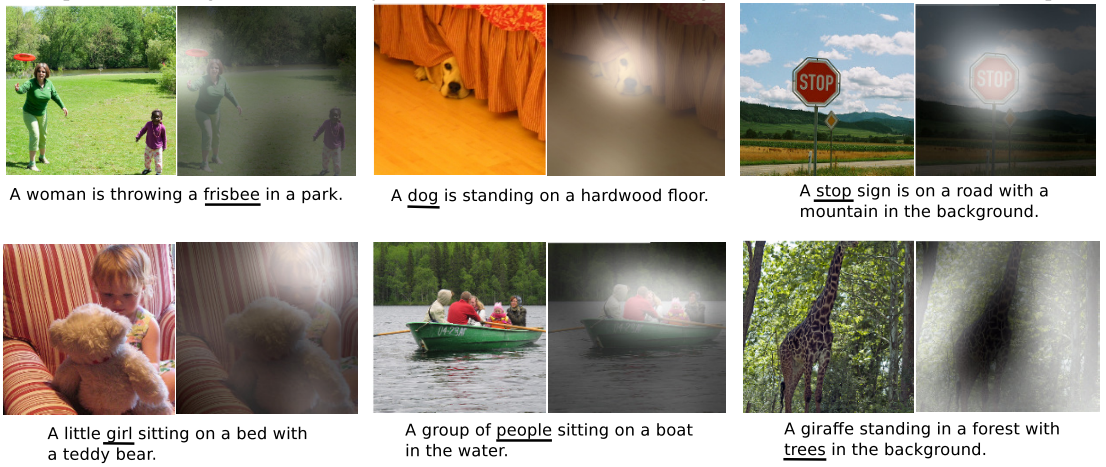
\includegraphics[width=\linewidth]{Xu2015.png}
  \caption{Caption generation with visual attention \cite{Xu2015}.}
\end{figure}

\begin{figure}[h!]
  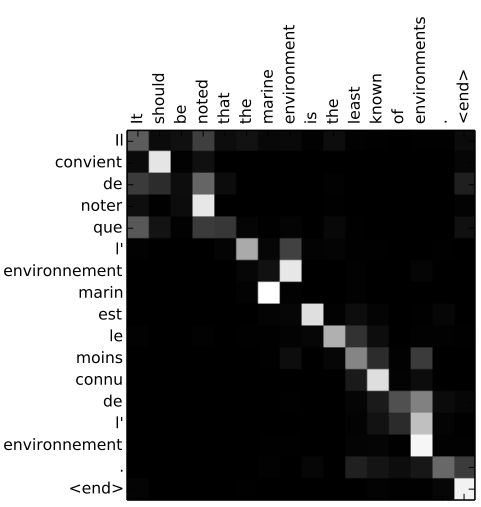
\includegraphics[width=\linewidth]{Bahdanau2015a.png}
  \caption{Alignment between source sentence (English) and generated sentence (French) \cite{Bahdanau2015a}.}
\end{figure}

\begin{figure}[h!]
  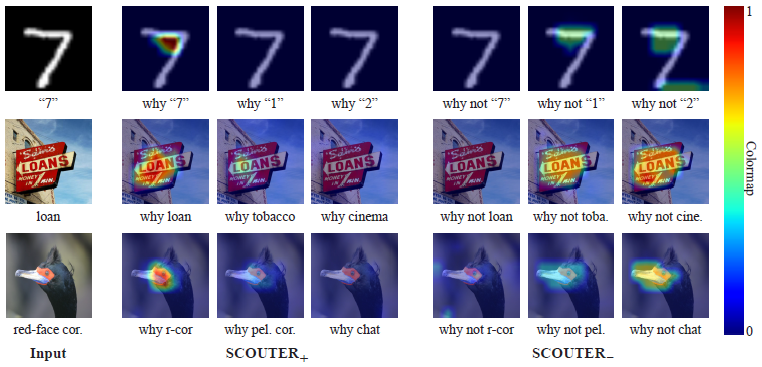
\includegraphics[width=\linewidth]{Li2020.png}
  \caption{Positive and negative attention-based explanations generated by SCOUTER \cite{Li2020}.}
\end{figure}

\cite{Brown2018} proposed an LSTM model for system log anomally detection that can be explained via an inherent attention mechanism. Given a value matrix $V_{(t)}$ that contains the LSTM hiddent states, a set of keys $K_{(t)}$ is computed for each log token: $K_{(t)}=tanh(V_{(t)}W^a)$, where $W^a$ are learned parameters. Then, the hidden states' attention values are calculated as: $a_{(t)}=softmax(q_{(t)}K^T_{(t)})V_{(t)}$, where $q_{(t)}$ is the query vector. Based on this, the probability distribution over the token at step $t$ is: $p_{(t)}=softmax([h_{(t-1)} \quad a_{(t-1)}]W+b)$.
\cite{Shu2019} developed an attention-based explainable framework that detects fake news by examining news sentences and user comments. Given the feature matrix of sentences $S=[s^1,...,s^N]$ and that of user comments $C=[c^1,...c^T]$, sentence and comment attention maps are calculated as: $H^s=tanh(W_sS+(W_cC)F)$ and $H^c=tanh(W_cC+(W_cS)F^T)$, where $F=tanh(C^TW_lS)$ and $W_l$, $W_s$, $W_c$ are weight parameters learned by the network. Based on these, the corresponding attention probabilities of each sentence and comment feature in $S$ and $C$ are computed as: $a^s=softmax(w_{hs}^TH^s)$, $a^c=softmax(w_{hc}^TH^c)$, where $w_{hs}$, $w_{hc}$ are weight parameters. The attended vectors $\hat{s}=\sum_{i=1}^Na_i^ss^i$ and $\hat{c}=\sum_{j=1}^Na_j^cc^j$ are then used for the model's prediction $\hat{y}=softmax([\hat{s},\hat{c}]W_f+b_f)$, where $W_f$ and $b_f$ are weight and bias terms.
\cite{Lu2020} proposed GCAN, a framework that uses the same dual co-attention mechanism to explain fake news detection. The main difference with the previous method is that, instead of utilizing user comments, GCAN examines the time propagation of user tweets that are triggered by the news source.
\cite{Yu2019} developed NAIRS, an attention-based explainable recommendation system. The attention value of each historical item $j$ is calculated as: 
$a_{uj}=\frac{exp(e(p_j))}{|\sum_{k \in R_u^+}exp(e(p_k))|^\beta}$, where $e(p_j)=V^Tg(W \cdot p_j+b)$ expresses the contribution of $j$ to the user's profile, $R_u^+$ is the user-item interaction matrix, $\beta$ is a smoothing hyper parameter, $V$ and $W$ are learned weights and $g(\cdot)$ is the activation function.
\cite{YingkaiGao2018} proposed an attention mechanism to interpret a deep learned drug-target interaction. Given $P$ and $D$, the context matrices of a protein and a drug respectively, a soft alignment matrix $A \in \mathbb{R}^{L_p \times L_d}$ is computed: $A=tanh(P^TUD)$, where $U$ is a learned parameter. Based on this, the attention weights that express the importance of the input units, are calculated as: $[a_p]_i=max_{1 \geq j \geq L_d}A_{i,j}$ and $[a_d]_j=max_{1 \geq i \geq L_p}A_{i,j}$. The final context vectors are then obtained as: $r_p=P \cdot softmax(a_p)$ and $r_d=D \cdot softmax(a_d)$, where $[softmax(v)]_i=\frac{e^{v_i}}{\sum_j e^{v_i}}$.
\cite{Li2020} introduced SCOUTER (Slot-based COnfigUrable and Transparent classifiER), a model that can replace a generic FC layer to produce explainable classifications based on multiple attention modules. Given a set of image features extracted by any network, SCOUTER calculates a feature subset that supports the decision towards or against a specific category.
\cite{Sha2017} developed an attentive neural network that predicts clinical outcomes based on the patient's medical data of past hospital visits. The model consists of two levels of bidirectional GRUs, each of which incorporates an attention mechanism to express the relative contribution of a visit to the model's prediction, as well as the importance of a given visit's record.
\cite{Chefer2021} introduced an attention-based Encoder-Decoder Transformer architecture for explainable VQA. The proposed model contains attention layers that generate relevancy maps indicative of the interactions between image and text inputs.
\cite{Zhang2017b} developed MDNet, an interpretable medical diagnosis network that utilizes an attention-augmented LSTM to learn a mapping between image features and word tokens of medical reports.
\cite{Li2021a} explains a CNN's predictions via applying attention maps on the input images. The attention values are obtained by calculating compatibility scores defined as the linear mapping from the set of feature vectors extracted at an intermediate layer to the output feature vector. 
Reverse Time AttentIoN (RETAIN) \cite{Choi2016} explains a prediction based on sequences of multifactor events, by training two RNNs in a reversed order to compute the appropriate attention components. 
\cite{Xu2015} implements a CNN to encode an input image to a context vector and an attentive LSTM to generate descriptive captions, where words reflect relevant parts of the image. In this way, the produced visualization indicates what the model is looking at when generating a word. 
In \cite{Bahdanau2015a}, an attention module is added to a neural machine translation model to allow the decoder to generate the ouput by iteratively focusing on different components of the input sentence. This technique allows the method to visualize language translation based on how respective words depend on each other. 

\begin{figure*}
\centering
\pgfkeys{/forest,
  rect/.append style   = {rectangle, rounded corners = 6pt, inner color = white},
  orect/.append style  = {rect, font = \rmfamily, text width = 325pt, text centered, minimum height = 10pt, inner color=white}}
\begin{forest}
    for tree={
      calign=edge midpoint,
      font=\rmfamily,
      line width=0.7pt,
      draw=black,
      rect,
      align=center,
      grow'=east,
      child anchor=west,
      parent anchor=east,
      drop shadow,
      l sep+=12.5pt,
      edge path={
        \noexpand\path[color=black, >={Stealth[length=7pt]}, line width=0.7pt, ->, \forestoption{edge}]
          (!u.parent anchor) -- +(10pt,0) |- (.child anchor)\forestoption{edge label};}
    }
    [{\makecell{xDNN\\methods}}
    [{\emph{When is it applicable?}}, calign=midpoint
      [Pre-model]
      [In-model]
      [Post-model]]
    [{\emph{Does it require} \\ {\emph{access to the model's}} \\ {\emph{internal components?}}}
      [Model-specific]
      [Model-agnostic]]
    [{\emph{Does it explain} \\ {\emph{a particular instance}} \\ {\emph{or the entire model?}}}
      [Local]
      [Global]]
    [{\emph{What is the} \\ {\emph{explainability's}} \\ {\emph{purpose?}}}
      [{\makecell{Prediction \\ explanation}}
        [Attribution-based
          [Attention]
          [Class activation mapping]
          [Distillation]
          [Gradients]
          [Inversion]
          [Perturbation]
          [Propagation]]
        [Evidence-based
          [Prototypes and Criticisms]
          [Counterfactuals]
          [Concepts]
          [Description]]]
      [{\makecell{Network \\ explanation}}
        [Preferred input]
        [Concept distribution]
        [Class distribution]
        [Information plane]]]
   ]
\end{forest}
\caption{Classification of xDNN methods}
\end{figure*}

\subsubsection{Class activation mapping}
\hfill\\
Class activation mapping is another attribution-based explanation technique, which has been developed to explain convolutional neural networks' predictions. The central characteristic of this family of methods is the computation of pixel importance heatmaps based on the CNNs' feature maps.

\begin{figure}
  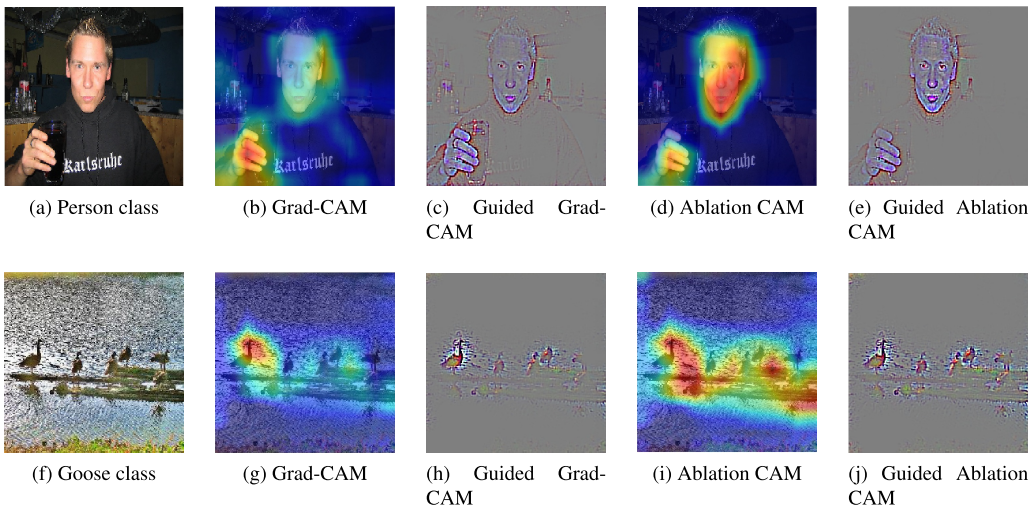
\includegraphics[width=\linewidth]{Desai2020.png}
  \caption{Ablation-CAM and Grad-CAM visualizations, along with their Guided form \cite{Desai2020}.}
\end{figure}

\begin{figure}
  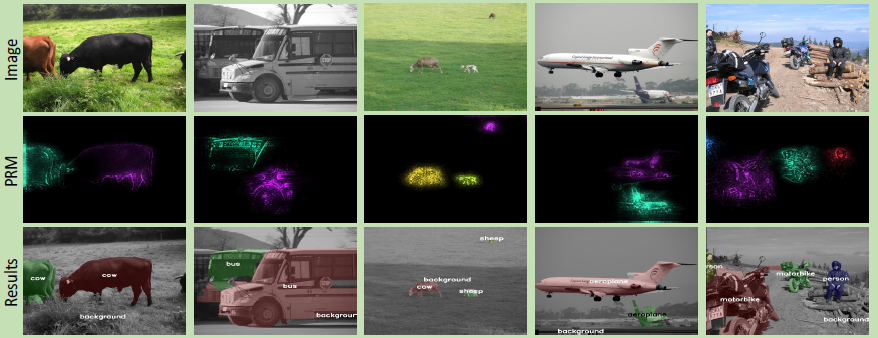
\includegraphics[width=\linewidth]{Zhou2018.png}
  \caption{Explanation generated by PRM \cite{Zhou2018}.}
\end{figure}

The original implementation of Class Activation Map (CAM) \cite{Zhou2016} computes the linear combination of $A^k$, the final feature maps of the convolutional network, weighted by $w_k^c$, the weight coefficients corresponding to unit $k$ for class $k$, to generate a saliency map that reflects the areas in the image that are strongly associated to the predicted classification class . The resulting map is thus given by: $L_{CAM}^c=\sum_kw_k^cA^k$. 
An important limitation of \cite{Zhou2016} is that it requires the model to employ a global average pooling (GAP) layer. To remove this constraint, Gradient-weighted Class Activation Map (Grad-CAM) \cite{Selvaraju2016} was developed as a generalization of the CAM method. Instead of employing the weights between the GAP layer and the fully connected output, Grad-CAM uses gradients as the weights to combine the different feature maps. For each feature map $A_k$ in the final convolutional layer of the network, a gradient of the logit $y_c$ of class $c$ with respect to every node in $A^k$ is computed and averaged to get an importance score $a_k^c$ for feature map $A^k$: $a_k^c=\frac{1}{m \cdot n}\sum_i\sum_j\frac{\partial y^c}{\partial A_{ij}^k}$ where $A_{ij}^k$ is a neuron positioned at $(i,j)$ in the m×n feature map $A^k$. Next, Grad-CAM linearly combines the importance scores of each feature map and passes them through a ReLU to obtain a $m\times n$-dimensional saliency map: $L_{Grad-CAM}^c=ReLU\left(\sum_ka_k^cA^k\right)$. 
In \cite{Selvaraju2016}, Guided Grad-CAM is also introduced as a combination of Grad-CAM with Guided Backpropagation through an element-wise product, in order to enhance the granularity of the produced explanation by obtaining pixel-scale representations. 
A limitation of the Grad-CAM method is that if there are multiple occurrences of an object or parts of an object that excite different feature maps, the final saliency map fails to highlight the presence of the object in all feature maps with equal importance. Grad-CAM++ \cite{Chattopadhay2018} addresses this problem by using a weighted average of the pixel-wise gradients. Specifically, the weights $w_k^c$ of the Grad-CAM methodology are reformulated as: $\sum_i\sum_ja_{ij}^{kc}ReLU\left(\frac{\partial y^c}{\partial A_{ij}^k}\right)$, where $a_{ij}^{kc}=\begin{cases} \frac{1}{\sum_{l,m}\frac{\partial y^c}{\partial A^k_{lm}}},& \text{if } \frac{\partial y^c}{\partial A_{ij}^k}=1\\ 0, & \text{otherwise} \end{cases}$. 
\cite{Omeiza2019} presents Smooth Grad-CAM++, a modified version of Grad-CAM++ that produces visually enhanced saliency maps by applying a smoothening technique in the gradients calculation. The first step is to generate n noised sample images by adding Gaussian noise to the original input. Followingly, the weight coefficients $a^{kc}$ are computed as: $a_{i,j}^{kc}=\frac{\frac{1}{n}\sum_1^nD_1^k}{2\frac{1}{n}\sum_1^nD_2^k+\sum_a\sum_bA_{a,b}^k\frac{1}{n}D_3^k}$, where $D_1^k$,$D_2^k$ and $D_3^k$ respectively denote the matrices of the \nth{1}, \nth{2} and \nth{3} order partial derivatives for feature map $k$ of all the noised inputs. The Grad-CAM++ weights $w_k^c$ then become: $w_k^c=\sum_i\sum_ja_{i,j}^{kc}ReLU\left(\frac{1}{n}\sum_1^nD_1^k\right)$. 
There also exists a gradient-free variation of the Grad-CAM method, called Ablation-CAM, which was developed in \cite{Desai2020}. Firstly, a component $y_k^c$ is obtained by setting all the individual cell values of feature map $A_k$ to zero and repeating the forward pass of the input. Then, similarly to Grad-CAM, Ablation-CAM is computed as: $L_{Ablation-CAM}=ReLU\left(\sum_kw_k^cA_k\right)$, where  $w_k^c=\frac{y^c-y_k^c}{y^c}$ expresses the slope of the activation score of class $c$ when feature map $A_k$ is removed. 
\cite{Wang2020} Score-CAM also removes the gradient dependence of the Grad-CAM method by calculating the weight of each feature map via its forward passing score on the outcome class. The final result is once more obtained by a linear combination of weights and feature maps. 
\cite{Bass2020} presents ICAM, a framework that improves class activation mapping via including a variance analysis module. Specifically, a VAE-GAN is employed to disentangle class relevance from background features that are shared between classes.    
\cite{Zhao2018} proposes Respond-weighted Class Activation Mapping (Respond-CAM) as an extension of the original CAM method for 3D images. Firstly, the importance coefficient of each feature map $A^l$ is computed as the weighted-average of all the gradients in the feature map using equation: $a_l^c=\frac{\sum_{ijk}A^l_{ijk}\frac{\partial y^c}{\partial A_{ijk}^l}}{\sum_{ijk}A_{ijk}^l+\epsilon}$, where $y^c$ is the classification score for class $c$,  $A_{ijk}^l$ stands for the position $(i, j, k)$ of the $l$-th feature map and $\epsilon$ is a sufficiently small positive number for numerical stability that can be usually ignored. Then the saliency map is computed by taking a linear combination of $A^l$ and $a_l^c$: $L_{Respond-CAM}^c=\sum_la_l^cA^l$. 
\cite{Meng2019} introduces a way to enhance the class activation mapping's localization (measured by the mean Intersection over Union value). Specifically, it proposes to generate the CAM as an average of the class activation maps of a small number of highly dissimilar classes. In the first step, the task's classes are divided into several clusters and representative classes from different clusters are selected. In the second step, given a class $c_i$ and its representative classes $s=\{s_1,...,s_N\}$, the activation maps by each binary classification task $(c_i,s_k)$ are calculated and then combined to generate the CAM. 
Inspired by CAM, \cite{Wolanin2020} proposed Regression Activation Mapping (RAM), an attribution method for CNN applied on time series data instead of temporal. The explanatory map is calculated as: $r_t=\sum_i^d z_{i,t}w_{z,i}$, where $\{z_{1,t},...,z_{d,t}\}$ are the input time seires to the GAP layer and $w_{z,i}$ are the weights of the ouput linear combination.
Furthermore, \cite{Zhou2018} developed Peak Response Map (PRM), a method that does not in essence belong to the CAM family but will be mentioned here in absense of a more fitting attribution-based technique group. The proposed algorithm proceeds as following. Given $M$, the class responce maps of the top convolutional layer, the location of the maps' peaks is computed. Next, for each class the corresponding peaks are backpropagated to the input image to obtain the class's peak response map and a respective segmentation mask is selected from a proposal gallery. This selection is based on the calculation of a resemblance score that takes into account the mask and both the class and peak responce map of the class. By assembling these visualizations for all detected classes, the objects that are present in the input image can be segmented and concurrently be attributed a specific class label.

\subsubsection{Distillation}
\hfill\\
Another common approach to attribution-based explainability methods is building surrogate models, also termed as model distillation. A surrogate model is an inherently interpretable model which is trained on the decisions of a complex model to mimic its input/output behavior \cite{Adadi2018}. The distilled model approximately imitates the qualities of the original model and is thus able to provide explanations fit to the statistical properties of the latter \cite{Du2018}. Examples of model types that can be used as surrogates are linear models, which can be interpreted based on their parameters, and rule-based, tree-based or graph-based models, whose structure can be utilized to trace their decision back to their input source \cite{Das2020}. 

\begin{figure}
  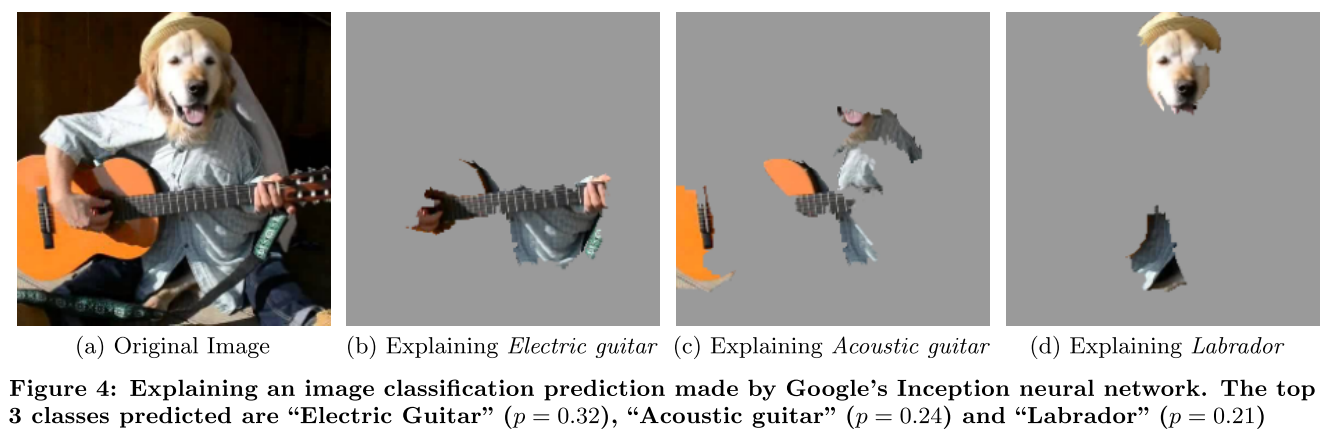
\includegraphics[width=\linewidth]{Ribeiro2016_a.png}
  \caption{Image classification explanation by LIME \cite{Ribeiro2016}.}
\end{figure}

\begin{figure}
  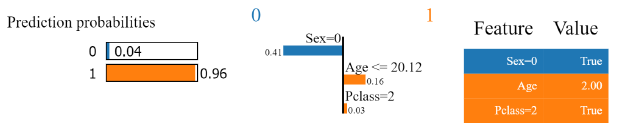
\includegraphics[width=\linewidth]{Gosiewska2019_a.png}
  \caption{LIME explanation for observation from Titanic data set. Blue color indicates the reasons for passenger’s death, orange indicates reasons for survival \cite{Gosiewska2019}.}
\end{figure}

\begin{figure}
  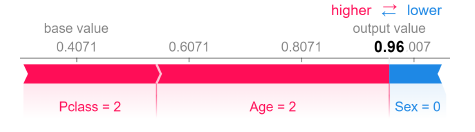
\includegraphics[width=\linewidth]{Gosiewska2019_b.png}
  \caption{SHAP explanations for observation from Titanic data set. Blue color indicates the features, which decrease probability of survival, red indicates features increasing this probability \cite{Gosiewska2019}.}
\end{figure}

\begin{figure}
  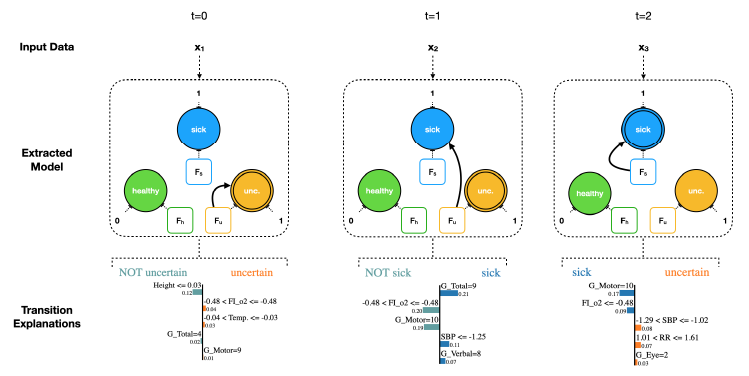
\includegraphics[width=\linewidth]{Kazhdan2020.png}
  \caption{Extracted sequence interpretation generated by \cite{Kazhdan2020}.}
\end{figure}

Following this approach, \cite{Ribeiro2016} proposed an explanation method called LIME (Local Interpretable Model-agnostic Explanations). LIME generates a new dataset by randomly perturbing sample data points in the neighborhood of the instance to be explained. Then it feeds this dataset to the target black-box model and uses its predictions, weighted by the proximity of the perturbed instances to the original ones, to train an inherently interpretable surrogate model, e.g. a decision tree or a linear regression model. \cite{Ribeiro2016} also introduced SPLIME, a LIME extension that provides global explanations of the model under study, using a submodular pick algorithm that is briefly described below. Given a set of instances X, SPLIME creates a matrix W of their corresponding explanations produced by LIME. Then, it computes the feature importance for each component of W and uses greedy optimization to choose a subset of X in a way that will include the most representative features detected by the original model. The size of this subset is selected as the number of explanations that the user is willing to observe to understand the model. 
Followingly, the authors of \cite{Ribeiro2016} developed Anchor Local Interpretable Model-Agnostic Explanations (aLIME) \cite{Ribeiro2016a}, a variation of LIME that provides model-agnostic interpretations of individual decisions in the form of if-then rules. These rules are produced in such a way that alterations in the rest of the input's parameters do not affect the model's decision with high probability.
Based on \cite{Ribeiro2016}, various methods have been developed to extend LIME in other tasks or to improve issues of the original method.
\cite{Mishra2017} develops Sound-LIME (SLIME), an extension of the LIME algorithm to music content analysis by temporal segmentation and frequency and time-frequency segmentation of an input spectrogram. 
In \cite{Peltola2018} the author proposes KL-LIME, a Kullback-Leibler divergence - based version of LIME that explains Bayesian predictive models. Similarly to LIME, local interpretable explanations are generated by projecting information from the predictive distribution of the original model to a simpler interpretable probabilistic explanation model, with respect to minimizing the KL-divergence between their decisions. 
Quadratic- LIME (QLIME) \cite{Bramhall2020} expands the linear relations of LIME to non-linear relationships, by considering the linear approximations as tangential steps within a complex function. 
\cite{Zafar2019} suggests an approach that enhances the stability of LIME algorithm. First, agglomerative Hierarchical Clustering (HC) is deployed to create groups of training data and the K-Nearest Neighbor (KNN) algorithm is used to find the closest neighboring cluster to the instance to be explained. Then, this selected cluster is passed as input to the perturbation step of the LIME algorithm and the computations continue as in the original method. 
GraphLime \cite{Huang2020} is an extended version of the LIME algorithm for deep graph models, that studies the importance of different node features for node classification tasks. Given a target node in the input graph, GraphLime considers the set of N-hop neighboring nodes and their predictions as its local dataset. Then a nonlinear surrogate model is created to fit the local dataset, using Hilbert-Schmidt Independence Criterion (HSIC) Lasso, a kernel-based feature selection algorithm. Finally, based on the weights of different features in HSIC Lasso, the most important features are selected and regarded as the explanations of the original GNN prediction. 
In \cite{Shi2020} the authors introduced Modified Perturbed Sampling operation for LIME (MPS-LIME), a variation of the LIME algorithm that considers the correlation between features, instead of generating perturbed samples from a uniform distribution. The authors formulate the picking procedure of the data points as a clique set construction operation, by converting the original image’s superpixels to an undirected graph. This formulation makes the method more time-efficient and enhances the understandability of the produced explanations. 
To reduce the time complexity, \cite{Elenberg2017} introduces STREAK, which is similar to LIME \cite{Ribeiro2016} but approaches the new dataset generation differently. Instead of randomly generating instances to train an interpretable linear model, STREAK directly selects critical input components by greedily solving a combinatorial maximization problem. In an image classification task for example, the input image which is predicted as a certain class by the original black-box model, is first segmented into superpixels via an image segmentation algorithm. Then, a superpixel set is iteratively formed to contain the parts of the image that maximize the probability of the opaque model to predict the given class and thus are the most important for the black-box model’s decision. This dataset is followingly used to create an interpretable surrogate model in a way similar to the LIME explanation method \cite{Ribeiro2016}.

Another explanation method that follows the distillation approach is SHAP (SHapley Additive exPlanations) \cite{Lundberg2017}, based on the Shapley Value \cite{Roth1988} developed for coalitional game theory to implement fair reward-sharing among cooperative participants. SHAP approximates the original model via a mechanism of additive feature attribution methods. Specifically, it builds a linear function of input features to obtain their relative contribution in the model’s decision. \cite{Lundberg2017} also proposes several variations of the baseline SHAP method: KernelSHAP reduces the multitude of evaluations required for large inputs, LinearSHAP estimates SHAP values from a linear model’s weight coefficients by assuming input feature independence, Low-Order SHAP is efficient for small maximum coalition size, Max SHAP reduces the complexity for the Shapley values computation of a max function, DeepSHAP employs DeepLIFT for the approximation of the SHAP values to improve computational performance by tapping into the compositional nature of deep neural networks. \cite{Aas2021} proposed an extension of KernelSHAP that explains the model's decision by combining individual Shapley values for groups of dependent features. \cite{Ghorbani2020} developed Neuron Shapley, a framework that utilizes SHAP to compute the contribution of neurons to the model's individual decisions, as well as general performance. \cite{Heskes2020} introduced causal Shapley values that calculate the contribution of input features to the model's prediction splitting their effect to direct and indirect. \cite{Frye2019} proposed Asymmetric Shapley values (ASVs), a variation of Shapley values that attends to consolidate any causal structure that may exist in the input data, by restricting the features' permutations during the SHAP calculation to the given causal ordering. \cite{Chen2019a} proposed L-Shapley and C-Shapley, two Shapley value variation approaches that achieve linear complexity when the data is graph-structured. L(ocal)-Shapley value is calculated by restraining the Shapley value to a neghbourhood of the target variable, whereas C(onnected)-Shapley value further limits the computation to regard only connected subgraphs of the local neighbourhood. \cite{Covert2020a} introduced Shapley Additive Global importancE (SAGE), a framework that combines the SHAP methodology with the notion of input features' predictive power, i.e. their exclusion's degrading effect on the model's prediction. In essence, SHAP is applied to the difference between the model's prediction loss when all features are considered and when a certain feature or subset of features is ignored. 

\cite{Bang2019} also proposes a distillation-based explanation method, the Variational Information Bottleneck for Interpretation (VIBI). VIBI adopts an information theoretic principle, the information bottleneck (analyzed later on in this survey), as a criterion for finding brief but comprehensive explanations. VIBI is composed of an explainer and an approximator, both modeled by a deep neural network. The explainer returns a vector of probabilities that indicate whether a chunk of features such as a word, phrase, sentence or a group of pixels will be selected as an explanation or not for each instance, and the approximator mimics the behaviour of the to-be-explained black-box model using the selected keys as the input. Using the information bottleneck principle, the explainer is trained to favor brief explanations by selecting key features that are maximally compressed about the input (briefness), while concurrently the explanations are enforced to suffice for accurate approximations to the black-box model by being informative about the output decision (comprehensive). 

Distilling a neural network to provide explanations of its decisions has further been implemented through the construction of graphs. 
In \cite{Yuan2020a}, the method XGNN is proposed to explain GNNs by  generating graph patterns that can maximize a prediction of the original graph model. This task is employed as a reinforcement learning problem. For each step the graph generator predicts how to add an edge to the current graph and then gets trained by feeding the generated graphs into the original GNN and receiving gradient policy feedback. The produced graphs are regarded as explanations for the target prediction and are expected to contain discriminative graph patterns. The validity and human-comprehensibility of these explanations is additionally enhanced by the incorporation of several graph rules. 
PGM-Explainer \cite{Vu2020} builds a probabilistic graphical model as a surrogate to provide explanations for GNNs. Given an input graph, PGM-Explainer randomly perturbs the node features of several random nodes within the computational graph and detects the influence of the perturbation on the GNN predictions. By repeating this procedure multiple times, a local dataset is obtained. Then, the dataset is reduced by selecting the top dependent variables using the Grow-Shrink (GS) algorithm. Finally, the local dataset is fitted by an interpretable bayesian network that is used to explain the predictions of the original GNN model. 
In \cite{Zhang2017} and the following \cite{Zhang2017a}, the authors propose to explain the knowledge hierarchy behind a convolutional network’s prediction, by building a semantic graph based on the CNN’s feature maps. The explanatory graph has a multilayer structure, much like CNNs. Each layer corresponds to a convolutional layer of the CNN and consists of many nodes, as every layer of the CNN consists of many filters. Each node represents a part pattern of the detected object, while the edges linking different nodes encode the latent spatial relationship between layers. It is also worth mentioning that every layer expresses different granularity, meaning that the larger object parts tend to be reflected in higher layers while smaller parts appear in lower layers. The proposed method can also be utilized as a network explanation method, as, along with explaining a prediction by localizing the most relevant parts of the image, it can also illuminate the overall relationship between the convolutional filters of a CNN and the parts of the objects it identifies.
\cite{Kazhdan2020} introduced MEME (Model Explanation via Model Extraction), a model extraction approach that distills RNNs to intepretable models resembling FSAs (Finite State Automata). Such a model is constructed via three steps: 1) the hidden space of a given RNN is approximated with a set of concepts that are extracted by summarizing clusters of the training data points' hidden states, 2) the transitions between these concepts are then approximated by a set of classifier functions, and 3) the concepts are mapped to the task's classes. At each timestep of the input sequence the produced MEME model calculates the next state from the current state and the next input token and outputs a class label based on this next state.

Another effort to gain insight into deep neural networks via surrogate models is the distillation of a DNN into a set of rules describing the logic behind its decisions. Works following this approach propose to extract rules that approximate the decision-making process of a trained network by utilizing its inputs and outputs. 
\cite{Andrews1995} includes an overview of mechanisms designed to extract rules from trained neural networks. It is worth noticing that the presented approaches are not generalizable as they strongly depend on the black box and on the specific type of decision rules. 
ANCHORS \cite{Ribeiro2018} uses sample inputs and outputs of a target model to generate a rule list that can be used to highlight the most influential input areas, so-called anchors. This can be achieved by starting from an empty set of rules and iteratively adding a rule for each feature predicate. Alternatively, the computation can start from a set containing all the possible candidate rules and then select the best ones in terms of precision. 
MUSE \cite{Lakkaraju2019}, which is an evolution of BETA \cite{Lakkaraju2017} by the same authors, also produces explanations by formulating decision sets. This framework allows end-users to customize the model explanations by inputting the features that interest them. Then, given the predictions of the target black-box model, MUSE generates a decision set based on an objective function that optimizes the explanations with respect to fidelity, interpretability, and unambiguity.    
LORE (Local Rule-Based Explanations) \cite{Guidotti2018a} distills the target model by learning a local inherently interpretable predictor on a neighborhood produced by a genetic algorithm. Then, based on this predictor, a set of rules is generated to explain the original model’s decision as well as suggest the changes in the input’s components that would result in a different output. 
\cite{GethsiyalAugasta2012} proposed a novel rule extraction approach that only takes into consideration the input neurons that were important for the classification.
Similarly, Genetic Rule EXtraction (G-REX) \cite{Konig2008} produces IF-THEN explanation rules by deploying genetic algorithms to create surrogate models, such as decision trees, kNN-rules, fuzzy-rules or regression models.
MAGIX (Model Agnostic Globally Interpretable eXplanations) \cite{Puri2017} also generates if-then rules to interpret the decision of a classifier by first extracting conditions that were important to the prediction and then running a genetic algorithm to build the explanatory set fo rules.
\cite{Letham2015} introduces Bayesian Rule Lists (BRL) a method that learns a decision list from a distribution using Bayesian techniques. Firstly, it creates a distribution of the most frequent rule patterns. Then, picking a sample rule list from this priori distribution, BRL optimizes the list by iteratively adding and editing the rules, in such a way that the new rule distribution follows the target posteriori distribution. 
\cite{Murdoch2017} approximates the performance of an LSTM model by building a rule-based classifier. After calculating an importance score for each word component of the output, the method selects the phrases that consist of the words with the higher joint importance. These extracted phrase patterns are then used in the rule-based classifier to approximate the output of the LSTM in an interpretable way.

Similarly to the rule extraction technique described above, surrogate models able to explain black-box systems, such as neural networks, can be implemented by the construction of decision trees. 
For example, Model Extraction \cite{Bride2018} generates decision trees via the Classification And Regression Trees algorithm (CART) and trains them based on a mixture of Gaussian distributions fit to the input data.
\cite{Liu2019a} also used CART to distill a DNN's decision process into a decision tree.
\cite{Che2016} proposed GBTmimic, a mimc learning approach that generates gradient boosting trees as interpretable surrogate models.
PALM \cite{Krishnan2017} distills a black-box model into a two-part surrogate model: a meta-model, constrained to be a decision tree, that partitions the training data, and a set of sub-models fitting the patterns within each partition. 
TreeView \cite{Thiagarajan2016} implements hierarchical partitioning of the feature space to construct a decision tree that represents the mechanics of a trained deep neural network.
\cite{Bastani2017} proposes to represent a black-box model’s behavior by generating decision trees based on the combination of logical conjunctions across paths from inputs to predictions and logical disjunctions across all the paths related to an output class.
In \cite{Zhang2019}, the authors train a decision tree that explains the percentage of contribution each input component has to the output decision. The building blocks of the decision tree are extracted via mining of semantic patters and “decision modes” from the target deep neural model. Nodes close to the top of the tree correspond to common modes shared by multiple instances, while nodes at the bottom represent fine-grained modes with respect to specific instances. 
\cite{Chatterjee2020} introduced a hybrid model that contains an LSTM that is used for the main classification task, as well as an XGBoost surrogate tree classifier that interprets the contribution of the input features to the LSTM's decision.
\cite{Bastani2017a} proposed to enhance the approximation achieved by a surrogate decision tree by actively sampling new training points during the extraction.
Instead of training a surrogate decision tree directly on the DNN's data, \cite{Frosst2018} proposed to use learned filters in the tree's training to obtain more informative targets.
\cite{Yang2019b} developed Global Interpretation via Recursive Partitioning (GIRP), an algorithm that, given a set of local instance-wise explanations, generates a surrogate tree that interprets a black-box model globally. To train the binary tree, input variables are averaged from the these explanations between divident spaces and their importance score difference is maximized through recursive partitions.

\subsubsection{Gradients}
\hfill\\
Attribution-based explanations can also be derived from some computation of the gradients of the model's output with respect to the input. The determined gradient-based values are regarded as approximations of the contribution of input features, elicited from the idea that larger gradient volume represents a more substantial sensitivity, and thus relevance, of a feature to the output decision. \cite{Du2018}

\begin{figure}
  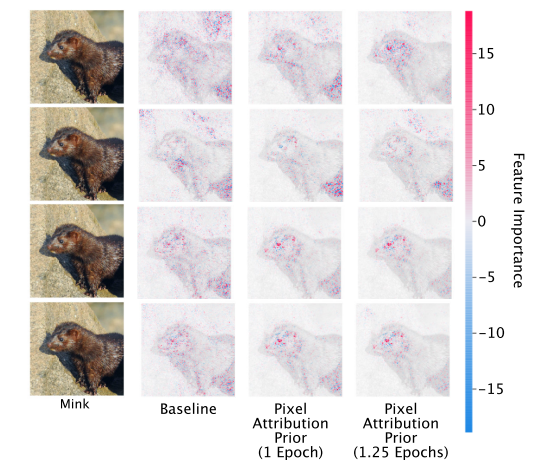
\includegraphics[width=\linewidth]{Erion2019.png}
  \caption{Attribution maps generated by Gradients, Gradients*Input, Integrated Gradients and Expected Gradients (top to bottom) before and after fine-tuning using an attribution prior \cite{Erion2019}.}
\end{figure}

Sensitivity analysis (SA) \cite{Simonyan2014} \cite{Baehrens2010} \cite{Li2016a} \cite{Yuan2019} \cite{Baldassarre2019} \cite{Vilamala2017} \cite{Leino2019}  \cite{Cortez2013} directly employs the squared values of gradients. Mathematically, it quantifies the importance of each input variable $i$ as $R_i=\left\| \frac{\partial f(x)}{\partial x_i} \right\|$. This value indicates how much a change in each input factor would a change the prediction $f$ in a small neighborhood around the input. It is assumed that the most relevant input features are those to which the output is most sensitive. 
The Global Sensitivity Analysis (GSA) method \cite{Cortez2011} extends the applicability of SA methods, allowing them for example to deal with discrete variables and distinct scanning functions.
Guided Backpropagation (GBP) \cite{Baldassarre2019} \cite{Springenberg2015} follows the same idea as Sensitivity Analysis but modifies the gradient backpropagation by restricting negative gradients from flowing back through ReLU units. This generally results in sharper explanations.
Gradient*Input (GI) \cite{Shrikumar2017} is a method that was initially introduced to enhance the display resolution of attribution maps. Explanations are produced by computing the partial derivatives of the output with respect to the input and element-wise multiplying them with the input itself: $R_i=\frac{\partial f(x)}{\partial x_i} \cdot x_i$. The input in this product acts as a smoothing filter that reduces the noise of the attribution. \cite{Ancona2017a} shows that Gradient*Input is equivalent to DeepLift and $\varepsilon$-LRP (methods analyzed in the following paragraph) for a network that contains only ReLUs and no additive biases. 
Similarly to Gradient * Input, Integrated Gradients (IG) \cite{Sundararajan2017} also utilizes the partial derivatives of the output with respect to each input feature. However, instead of computing a single derivative evaluated at the provided input x, Integrated Gradients integrates the gradient of the model function at all points along the straight-line path from a baseline input $x’$ (usually a zero matrix or vector) to $x$: $IG_i(x)=(x_i-x_i') \int_0^1 \frac{\partial f(x'+a(x-x'))}{\partial x_i}da$, where $i$ describes the dimension along which the gradient is calculated and $a$ is associated with the path from $x$ to $x’$ and is smoothly distributed in range $[0,1]$. Integrated Gradients is in essence a smooth version of Gradient * Input and reduces to the latter when the function is linear on the integration domain.
Built on Integrated Gradients, \cite{Kapishnikov2019} introduced XRAI, a method that improves attribution in cases when the image is not well fixed towards the object of interest. To achieve this, XRAI segments the input image to many overlapping parts of varrying contours and then fuses smaller regions to larger segments based on their IG-based attribution importance.
Furthermore, as a substitute for Integrated Gradients that removes the influence of the selected baseline, \cite{Erion2019} introduced Expected Gradients (EG): $EG(x)=\int_{x'}\left ((x_j-x_j')\int_0^1\frac{\partial f(x'+a(x-x'))}{\partial x_j}da\right ) \cdot p_D(x')dx'$, where $D$ is the distribution of the underlying data domain.
\cite{Xu2020} proposed another variation of Integrated Gradients, called Blur Integrated Gradients (BlurIG), that obtains the integration path by successively blurring the input via a 2D Gaussian blur filter. Based on this idea, the integration is computed as: $BlurIG(x) = \int_{a=\infty}^0 \frac{\partial f(L(x,a))}{\partial L(x,a)} \frac{\partial L(x,a)}{\partial a} da$, where $L(x,a)$ is the convolution of the input with the Gaussian kernel. This is claimed to produce sharper heatmaps by producing localization ''in both scale/frequency and space''.
\cite{Janizek2021} developed Integrated Hessians, an extension of Integrated Gradients that takes into account the interactions between the features within the neural model. Specifically, this method computes the importance of input feature $i$ with respect to the feature $j$ as: $\Gamma_{i,j}(x)=(x_i-x_i')(x_j-x_j') \int_{\beta=0}^1 \int_{\alpha=0}^1 \alpha \beta \frac{\partial ^2 f(x'+\alpha \beta (x-x'))}{\partial x_i \partial x_j}d\alpha d\beta$.
To achieve more precise confinement of the produced heatmap around the localized object, \cite{Srinivas2019} developed another gradient-based method, named Full-Gradient. Given a ReLU neural network $f(x,b)=\nabla_x f(x,b)^Tx+\nabla_b f(x,b)^Tb$, where $b$ are its biases, $\nabla_x f(x,b)$ is defined as the input-gradient and $\nabla_b f(x,b) \odot b$ as a bias-gradient. Based on these, FullGrad aggregates the input-gradient with bias-gradients of intermediate layers to produce the final FullGrad heatmap.
As an improvement for the above type of methods, SmoothGrad \cite{Smilkov2017} was developed, a technique that can utilize any gradient-based method and produce a sharper, more accurate attribution map. Specifically, SmoothGrad alleviates noise by averaging out the explanations over a batch of noisy copies of the input. Given an explanation E, SmoothGrad is defined as $E_{sg}(x)=\frac{1}{N}\sum_{i=1}^N E(x+g_i)$, where noise vectors $g_i \sim N(0,\sigma^2)$ are drawn from a normal distribution.
There is also a variance analog of SmoothGrad, VarGrad introduced in \cite{Sundararajan2018}, that aggregates the noisy estimates by computing the variance of the noisy set rather than the mean: $E_{vg}(x)=Var(E(x+g_i))$.

\subsubsection{Inversion}
\hfill\\
Inversion is another attribution-based technique, which has been developed to explain deep convolutional networks. Its key idea is to approximately reconstruct the original image from intermediate layers’ feature maps and project the inverse representation on the input image as a heatmap. The motivation of this approach is to reveal what image information is preserved in the inner layers, as it is assumed that the convolutional layers mainly consider the features that are relevant for the network’s decision. \cite{Vilone2020}

\begin{figure}
  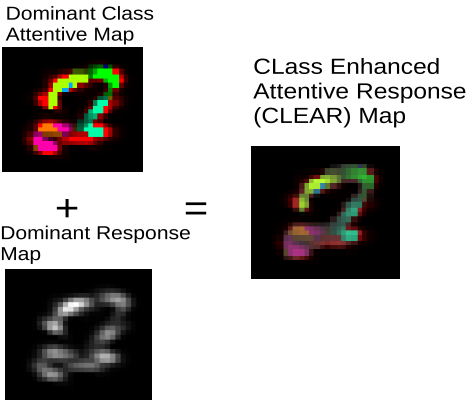
\includegraphics[width=\linewidth]{Kumar2017.png}
  \caption{Visual explanation maps generated by CLEAR \cite{Kumar2017}.}
\end{figure}

\begin{figure}
  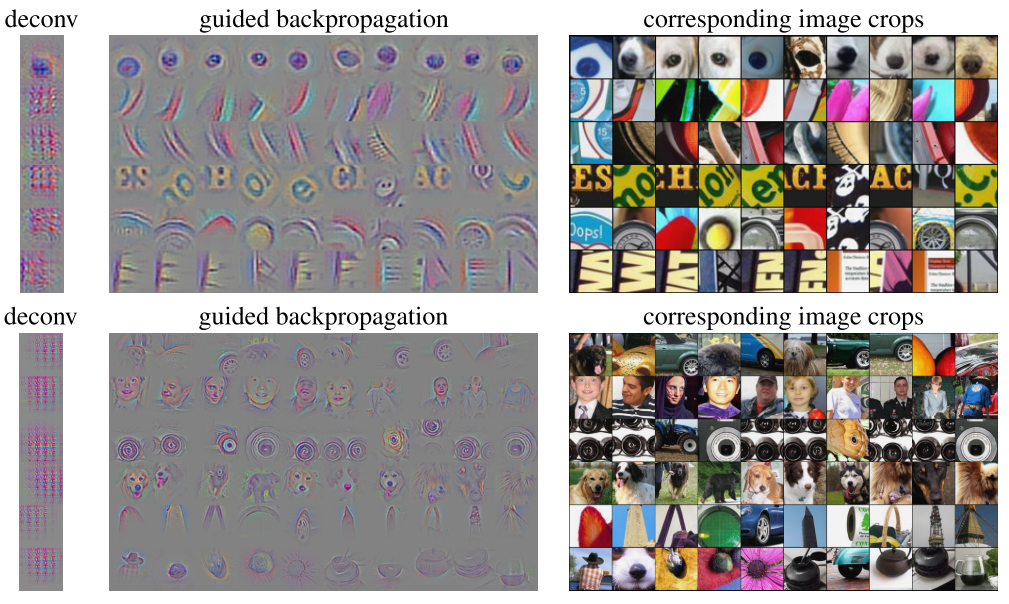
\includegraphics[width=\linewidth]{Springenberg2015.png}
  \caption{Visualization of patterns learned by the layer conv6 (top) and layer conv9 (bottom) of a network. Each row corresponds to one filter \cite{Springenberg2015}.}
\end{figure}

\begin{figure}
  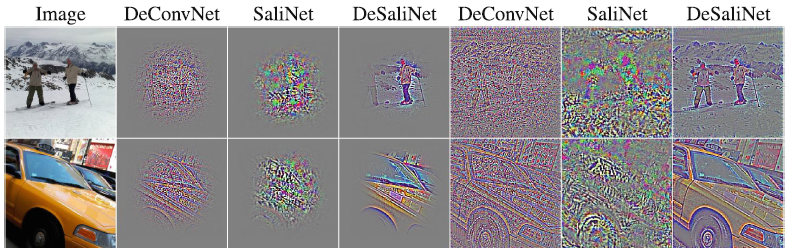
\includegraphics[width=\linewidth]{Mahendran2016a.png}
  \caption{Comparison of DeconvNet with DeSaliNet \cite{Mahendran2016a}.}
\end{figure}

\cite{Mahendran2015} \cite{Mahendran2016} propose to reconstruct the image from each layer by using gradient descent and a regularization term. It uses the same architecture and parameters as the original CNN before the visualization target layer and adjusts each pixel of the to be reconstructed image to minimize the objective loss function error between the target reconstruction feature map and the feature map of the original input image.
\cite{Dosovitskiy2016} \cite{Dosovitskiy2017} reconstruct the image by training a dedicated Up-convolutional Neural Network (UpconvNet). The UpconvNet computes an inverse path for the feature maps back to the image dimension. The parameters of the UpconvNet are adjusted to minimize the objective loss function error between the reconstructed image and the original input image.     
Guided Feature Inversion \cite{Du2018a} generates an inverted image representation consisting of the weighted sum of the original image and another noisy background image, i.e. a Gaussian white noise image. The weights are calculated to highlight the smallest area that contains the most relevant features and to blur out everything else. 

Another form of inversion, that can illuminate the image information that a CNN detects, is deconvolution.
In \cite{Zeiler2010}, the authors proposed a deconvolutional neural network structure, referred to as DeconvNet, aiming to capture certain general features for reconstructing the original image by projecting a highly diverse set of low-dimension feature maps to high dimension. DeconvNet implements the inverse operations of a CNN, consisting of reversed convolutional layers (namely the deconvolutional layer), reversed rectification layers, and reversed max-pooling layers (namely unpooling layer) in the DeconvNet structure. 
Then, in \cite{Zeiler2011} they utilized the DeconvNet structure to decompose an image hierarchically from low-level edges to high-level object parts.
However, the method gained popularity when \cite{Zeiler2014} proposed its application on visualizing higher layer features in the input space, in other words mapping hidden features on pixels, to shed light into the learned activation of convolutional layers. 
Central to the \cite{Zeiler2014} method are discriminative patterns encoded in the max pooling layers of the network, that contain the information about which pixels in the input space are of the highest importance for the resulting feature activations. \cite{Springenberg2015} surpassed this limitation, generalizing the DeconvNet to also work with networks that do not have max pooling layers.
Proceeding in this direction, \cite{Mahendran2016a} introduced DeSaliNet via combining the DeconvNet architecture with the sensitivity analysis of \cite{Simonyan2014} to enhance the resulting heatmap's localization.
Utilizing the above deconvolutional approaches, Relevant Features Selection was developed in \cite{JoseOramas2017}. This method uses a two-step algorithm to identify the internal features of a neural network mostly relevant for the prediction. First, a set of relevant layer/filter pairs are identified for every class of interest by finding those pairs that reduce at the minimum the differences between the predicted and the actual labels. These relevance values are elementwise multiplied with the internal filter-wise response vectors to obtain the contribution scores of the layer/filter pairs that are most important for the prediction. Then, this information is fed to the Deconvnet-based visualization method described in \cite{Grun2016} to generate an explanation heatmap.
One more method that interprets convolutional neural networks based on the work of \cite{Zeiler2010} is CLass-Enhanced Attentive Response (CLEAR) \cite{Kumar2017}. By performing deconvolution on the network's last layer, CLEAR produces attribution maps that not only facilitate the visualization of the attentive regions mainly responsible for the prediction, but also the class that has the dominant influence on each pixel of these regions.

\subsubsection{Perturbation}
\hfill\\
Among the attribution-based explanation methods, there is also a line of work built on the notion that measuring how the outcoming prediction is affected by alterations of a feature can reflect this feature's contribution \cite{Du2018}. This technique is referred to as perturbation and it practically suggests to determine the attribution of an input feature or set of features by removing, masking or modifying them, computing the output on this new input and measuring the difference with the original output \cite{Ancona2017}. Previously discussed methods PGM-Explainer, LIME and SHAP use this technique to construct their surrogates.

\begin{figure}
  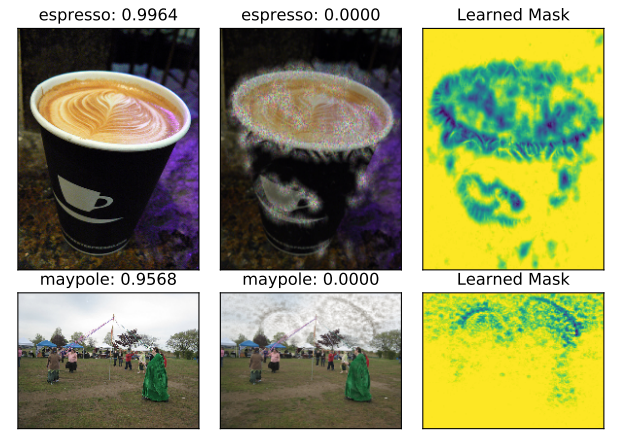
\includegraphics[width=\linewidth]{Fong2017.png}
  \caption{An image correctly classified with large confidence; a perturbed image that is not recognized correctly anymore; the deletion mask \cite{Fong2017}.}
\end{figure}

\begin{figure}
  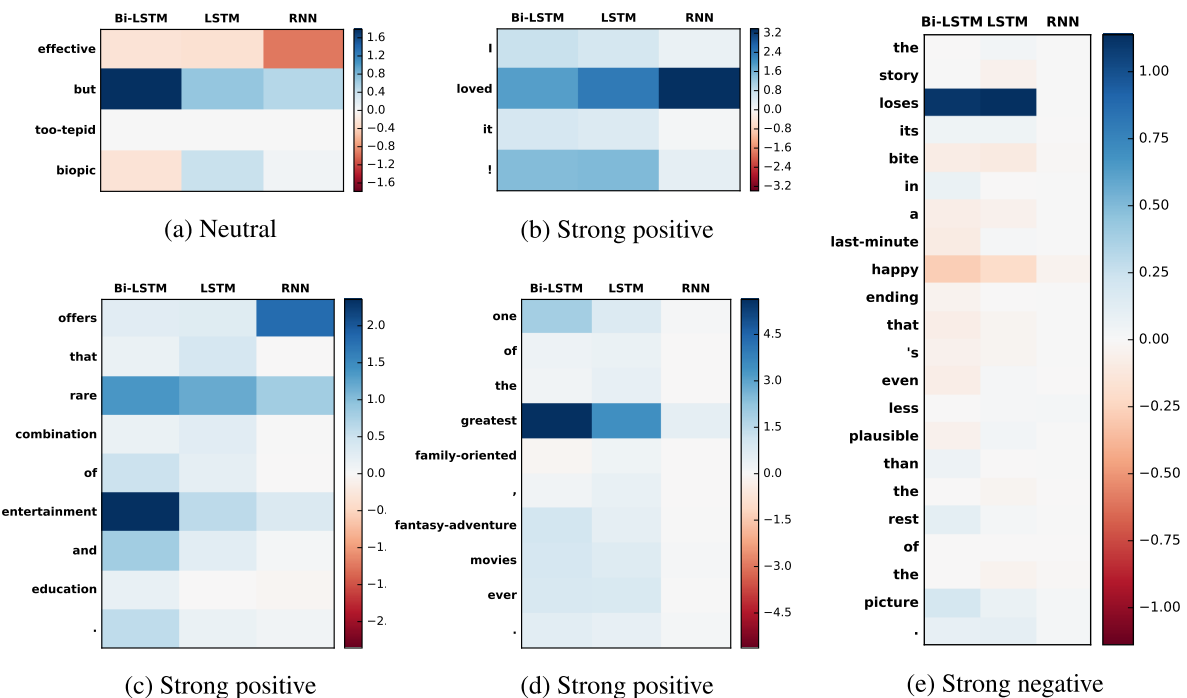
\includegraphics[width=\linewidth]{Li2016_a.png}
  \caption{Heatmap of word importance in sentiment analysis generated by Representation Erasure \cite{Li2016}.}
\end{figure}

Explain \cite{Robnik-Sikonja2008} was developed to calculate the contribution of a particular input variable by hiding its actual value and measuring the difference between the output probability scores predicted with the altered and the original input, $p(c|x_{-i})$ and $p(c|x)$ respectively. The marginal probability $p(c|x_{-i})$ is calculated as $p(c|x_{-i})=\sum_{x_i} p(x_i|x_{-i})p(c|x_{-i},x_i)$, where $x$ denotes all input features, $x_{-i}$ denotes all features except $x_i$, and the sum iterates over all possible values of $x_i$. Then, the prediction difference is calculated by $Diff_i(c|x)=log_2(odds(c|x))-log_2(odds(c|x_{-i}))$, where $odds(c|x) = \frac{p(c|x)}{1-p(c|x)}$. 
However, the one-variable-at-a-time approach of Explain often results in unintuitive explanations, as it ignores the redundancies between input features. Attending to this weakness, \cite{Strumbelj2009} proposed Ime, a variation of Explain that observes all subsets of input variables. 
\cite{Zintgraf2016} also proposed a variation of Explain that replaces $p(x_i|x_{-i})$ with $p(x_i|\hat{x}_{-i})$, where $\hat{x}_{-i}$ contains only the pixels surrounding $x_i$ instead of including all pixels except $x_i$. 
Followingly, Prediction Difference Analysis (PDA) \cite{Zintgraf2017} was developed, also based on Explain. Instead of assessing the contribution of a feature, in this case pixel, at a time, PDA considers patches of pixels to atone the high dependence that each pixel has on the surrounding pixels. The patches are overlapping so that, ultimately, an individual pixel’s relevance is calculated as the average relevance of the different patches it was in.   
\cite{Seo2020} proposed a variation of PDA that, instead of using rectangular patches, performs segmentation of the input image at multiple scales. The importance of each of these parts is then calculated in a way similar to PDA.
Occlusion Sensitivity is another method following the perturbation approach, which was introduced in \cite{Zeiler2014} discussed in the previous paragraph. It works by sweeping a grey patch that occludes pixels over the image and sees how the model prediction and/or the hidden layers’ activation varies as the patch is covering different positions. When the patch covers a critical area the prediction performance drops significantly. Based on this notion, the method produces a visualization that depicts the most sensitive areas of an image with respect to its classification label and/or one or more intermediate layers.
Representation Erasure \cite{Li2016} is an analogous explanation method that was developed for the natural language processing (NLP) domain. It measures the importance of each input word or each dimension of intermediate hidden activations by deleting the word or zeroing the dimension correspondingly and observing the influence on the model prediction. The influence of multiple words or phrases combined is also evaluated with the use of reinforcement by finding the minimum changes in the text that cause a flipping of the network’s decision.   
Similarly, \cite{Jin2019} proposed Sampling and Occlusion (SOC), an algorithm that estimates the importance of input components for an NLP classification decision, by observing the prediction difference: $\phi(p,x)=s(x)-s(x_{-p};0_p$, caused by replacing words or phrases $p$ with padding tokens $0_p$.
Meaningful Perturbation \cite{Fong2017} produces explanations in the forms of saliency maps by omitting information from different areas of the image and checking the resulting change in the output. The authors define three kinds of perturbations to delete information: i) constant, replacing a region with a constant value ii) noise, adding noise to the region, and iii) blur, blurring the region area. 
To this approach, \cite{Fong2019} introduced an algorithm that, having found the mask that maximizes the model's ouput, optimizes its bound to obtain the smallest mask that causes at least this output level. In this way, the visualization confines the object of interest more accurately.
\cite{Dabkowski2017} is a CNN explanation method that generates masks similarly to Meaningful Perturbation but considering SDR (Smallest Destroying Region, i.e. the minimal image region that when ommited leads the model to a false classification) along with SSR (Smallest Sufficient Region, i.e. the minimal region that is sufficient for the model to result in the correct classification) in the objective that is being optimized. The main difference however is that instead of generating the masks iteratively which has high time requirements, a novel masking model is trained to create the masks in a single forward pass.
Permutation Feature Importance \cite{Altmann2010} also measures the importance of each specific feature of a deep model to the overall performance by calculating how the prediction accuracy deviates after permuting the values of that feature. 
Randomized Input Sampling for Explanation (RISE) \cite{Petsiuk2018} perturbs an input image by multiplying it with randomized masks. The masked images are then fed to the black-box model and the scores of the target class corresponding to the masked inputs are used as coefficients to compute a weighted average of the respective masks. This sum is returned as a heatmap that indicates the important image areas for the specific prediction.
\cite{Sattarzadeh2020} introduced Semantic Input Sampling for Explanation (SISE), a modified version of RISE, that uses non-random sampling to avoid instability issues. SISE is implemented in three main steps: 1) A set of feature maps is extracted from a layer of the convolutional model. 2) From this set, the most important maps are selected based on the gradient of the model's output with respect to each of them. 3) These feature maps are processed to generate targeted perturbation masks that are used in place of the random ones in the RISE methodology. Steps 1-3 are applied to multiple layers and the resulting saliency maps are aggregated to obtain the final explanation map.
\cite{Alvarez-Melis2017} provides explanations in the form of partitioned dependency graphs, produced in three main steps. The first step involves sampling perturbed versions of the data using a VAE. The second step uses the perturbed input-output pairs to determine dependencies between the original input and output tokens. The last step selects the explanation sets.
\cite{Datta2017} introduces Quantitative Input Influence (QII), a set of perturbation-based measures that indicate the influence of input features on the output of a black-box model. 
\cite{Arrieta2021} proposed a method to explain Deep Echo State Networks via measuring the ''pixel absence effect'', in other words by observing the output difference caused by zeroing an input data point, which might be either a pixel or a point of the input sequence for image/video and time series classification tasks respectively.
GNNExplainer \cite{Ying2019} uses masks for edges and node features to identify a compact subgraph structure and a small dataset of features that are mostly responsible for a GNN’s prediction. The masks are randomly initialized and their optimization is implemented by maximizing the mutual information between the predictions of the original graph and the predictions of the generated masked graph.  
PGExplainer \cite{Luo2020} explains a GNN's predictions via edge masks that are produced by training a parameterized mask predictor. Given an input graph, the predictor first obtains the embeddings for each edge by concatenating node embeddings. Then the predictor uses the edge embeddings to compute the probability of each edge to be selected, which is considered as the importance score of each edge. Next, the approximated masks are sampled and applied to the graph. Finally, the mutual information between the new and the original predictions is maximized to train the predictor. 
GraphMask \cite{Schlichtkrull2020} explains edge importance in graph networks, by generating an edge mask for each GNN layer. It trains a classifier to predict whether an edge can be dropped without affecting the original predictions. To avoid changing the graph structure, the dropped edges are replaced by learnable baseline connections, which are vectors with the same dimensions as the node embeddings. The classifier is trained using the whole dataset by minimizing a divergence term, which measures the difference between network predictions. 
Contrastive Explanations Method (CEM) \cite{Dhurandhar2018} utilizes a convolutional autoencoder (CAE) to compute the minimal amount of features that need to be present for the model to result in the same prediction (''pertinent positives''), as well as the minimal amount of features that should be absent to mantain the classification result (''pertinent negatives''). Thanks to the use of the CAE, the inflicted perturbations are closer to the data manifold, hence resulting in more human comprehensible explanations.
SImilarity Difference and Uniqueness Method (SIDU) \cite{Muddamsetty2020} is another visual explanation approach that utilizes the notion of masking the model's input image to estimate pixel saliency. Each feature activation map is converted into a binary mask $M_i^c$ that gets bi-linearly interpolated to match the size of the input image $I$. The produced mask is element-wise multiplied with $I$ resulting in a set of perturbed images $A_i^c$. Each $A^c$ is then fed to the CNN model to calculate the corresponding probability prediction scores $P_i^c$. Based on these and the probability prediction score for the original image, $P_{org}^c$, similarity difference and uniqueness values are computed for each feature: $SD_i^c=exp(\frac{-1}{2\sigma^2}\lVert P_{org}^c-P_i^c \rVert)$ and $U_i^c=\sum_{j=1}^N \lVert P_i^c-P_j^c \rVert$ respectively. The final explanatory heatmap of the CNN's prediction is then obtained as: $S_c=\frac{1}{N}\sum_i^NW_i^c \cdot A_i^c$, where $W_i^c=SD_i^c \cdot U_i^c$.
\cite{Alvarez-Melis2017} developed a framework that returns causally related input and output tokens. Inputs are perturbed by a variational autoencoder and the black-box model's prediction for each of the new instances is used to create an input-ouput graph. A partitioning problem can then be solved to highlight the most important input tokens.
\cite{Burns2020} observes the model's prediction difference when input features are replaced with ''uninformative'' counterfactuals.
\cite{Chang2019} proposed an enhancement for perturbation-based methods that calculate the importance of an image part feature via heuristic occlusion, e.g. via blurring it or replacing it with noise. Instead, the paper proposes to use a generative model, conditioned, on the rest of the image, that removes the part of interest in a way that respects its relationship with neighbouring image regions. In this way, the perturbed instances are more realistic, thus resulting in more compact and comprehensive explanations.
\cite{Agarwal2021} developed another generative ''in-filler'' for the same cause.
\cite{Wagner2019} proposed a masking perturbation approach that produces two types of explanations: ''Explanation by Preservation'', which indicates the minimal region of the original image that is needed for the model to result in the same prediction, and ''Explanation by Deletion'', that highlights the minimal region that must be deleted to alter the model's output.
\cite{Yuan2020b} introduced a maks generator that learns to locate image regions that are discriminative for a deep classifier's prediction. The generator produces a probability map from which a discrete mask can be sampled. The masked input image is then fed to the deep model and the cross entropy between the new and the original output is calculated to train the generator.
\cite{Schwab2019} proposed CXPlain, a method that trains a seperate explanation model to interpret a predictive model by estimating the contribution of either a single input feature or a group of features to the model's accuracy. For each training data instance, the model's prediction loss when considering all available input features is calculated, as well as the loss when the target input feature's information is excluded. The normalised difference between these two losses is regarded as the importance score of the feature and the explanatory model is trained to approximate this target importance distribution.
\cite{Guan2019} proposed a perturbation-based method for NLP tasks, that estimates the information contained in a word in the hidden states of a deep model's intermediate layers. This is achieved by calculating the change in the hidden state's confidence when replacing the target word with other random words.

\subsubsection{Propagation}
\hfill\\
Another mechanism that is commonly employed in attribution-based methods is decomposition with propagation rules. This approach is constituted by progressively redistributing the output backwards layer by layer. Considering the model’s prediction as the initial target score, this score is decomposed and distributed to the neurons in the previous layer following the propagation rules. By repeating such procedures until the input layer, importance scores for each node of the neural network can be obtained. \cite{Yuan2020}

\begin{figure}
  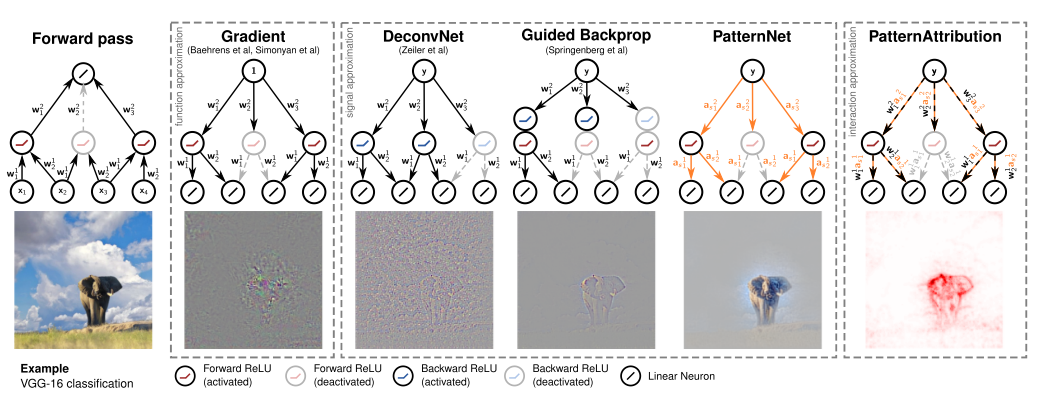
\includegraphics[width=\linewidth]{Kindermans2018.png}
  \caption{Heatmaps of pixel-wise contributions \cite{Kindermans2018}.}
\end{figure}

\begin{figure}
  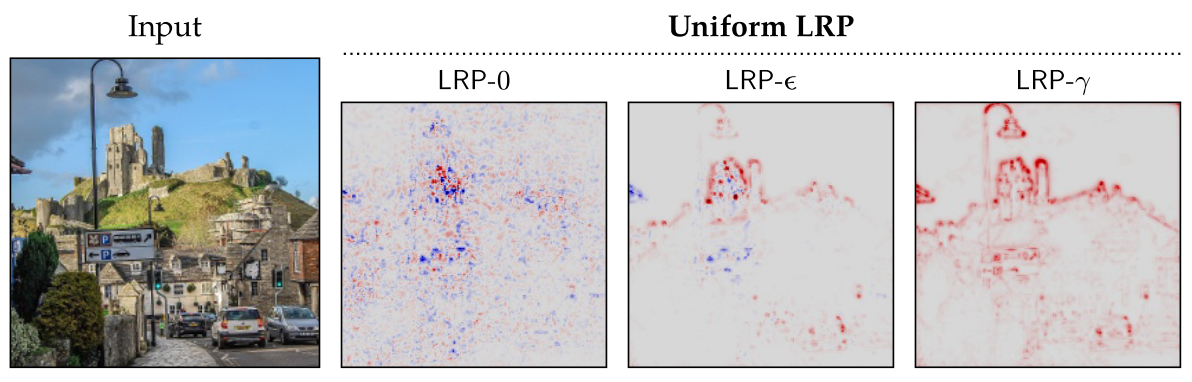
\includegraphics[width=\linewidth]{Montavon2019.png}
  \caption{Pixel-wise explanations of the output neuron ‘castle’ obtained with various LRP procedures. \cite{Montavon2019}.}
\end{figure}

\begin{figure}
  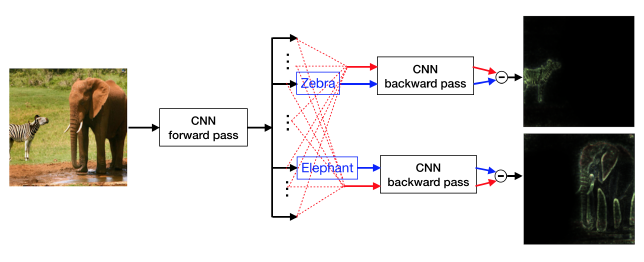
\includegraphics[width=\linewidth]{Gu2019.png}
  \caption{Explanation generated by CLRP \cite{Gu2019}.}
\end{figure}

\begin{figure}
  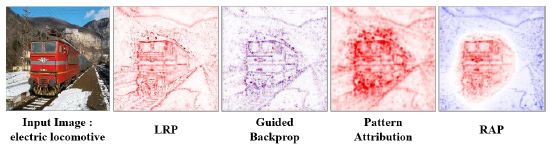
\includegraphics[width=\linewidth]{Nam2020.png}
  \caption{Comparison of conventional propagation explanations to RSP \cite{Nam2020}.}
\end{figure}

\begin{figure}
  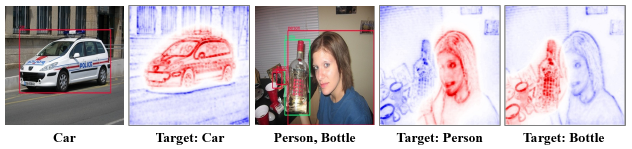
\includegraphics[width=\linewidth]{Nam2020a.png}
  \caption{Explanations generated by RSP \cite{Nam2020a}.}
\end{figure}

Deep Learning Important FeaTures (DeepLIFT) \cite{Shrikumar2017a} computes the contribution scores of features based on the difference between the original activation of each neuron and a ‘reference activation’ value computed by propagating a ‘reference input’ (e.g. a white image) through the network. In more detail, DeepLIFT assigns a relevance score $R_{\Delta x,\Delta t}$ for input feature $x_i$ such that: $\Delta t=\sum_{i=1}^NR_{\Delta x_i,\Delta t}$, where $N$ is the number of input neurons that are necessary to compute $t$, $\Delta t=f(x)-f(x')$ is the difference-from-reference of an interested neuron output of the network between $x$ and reference $x’$, and $\Delta x=x-x'$ is the difference between $x$ and $x'$. In this formulation, $R_{\Delta x_i,\Delta t}$ can be thought of as a weight denoting how much influence $\Delta x_i$ had on $\Delta t$. This relevance score can be calculated via the Linear rule, Rescale rule, or RevealCancel rule, described in the paper. A multiplier  $m_{\Delta x,\Delta t}$ is defined as $m_{\Delta x,\Delta t}=\frac{R_{\Delta x,\Delta t}}{\Delta x}$ indicating the relevance of $\Delta x$ with respect to $\Delta t$, averaged by $\Delta x$. Given a hidden layer $l$ of nodes $a^l=(a_1^l,a_2^l,…,a_K^l)$, whose upstream connections are the input nodes $x=(x_1,x_2,…,x_N)$, and a downstream target node is $t$, the DeepLIFT paper proves the effectiveness of the chain rule: $m_{\Delta x,\Delta t}=\sum_{j=1}^Km_{\Delta x_i \Delta a_j^l}m_{\Delta a_j^l \Delta t}$. This chain rule allows for layer-by-layer computation of the relevance scores of each hidden layer node via backpropagation. The DeepLIFT paper and appendix specify particular rules for computing $m_{\Delta x_i \Delta a_j^l}$ based on the architecture of the hidden layer $a^l$. 

Layer-wise Relevance Propagation (LRP) \cite{Bach2015} \cite{Montavon2018} \cite{Montavon2019} was proposed as a method for pixel-wise decomposition of relevance to a decision. Mathematically, it redistributes the prediction $f(x)$ backwards using local redistribution rules until it assigns a relevance score $R_i$ to each input variable. The Relevance conservation is the key property of the redistribution process and can be summarized as $\sum_iR_i=...=\sum_jR_j=\sum_kR_k=...=f(x)$. This property ensures that no relevance is artificially added or removed during redistribution. The relevance score $R_i$ of each input variable determines the variable's contribution to the prediction. A general propagation rule is given by: $R_j=\sum_k \frac{a_j \cdot (w_{jk}+\gamma w_{jk}^+)}{\epsilon + \sum_{0,j}a_j \cdot (w_{jk}+\gamma w_{jk}^+)}R_k$, where $a_j$ is the neuron activations at layer $l$, $R_j$ and $R_k$ are the relevance scores associated to the neurons at layer $l$ and $l+1$ respectively, $w_{jk}$ is the weight connecting neuron $j$ to neuron $k$ and $\gamma$, $\epsilon$ are hyperparameters to be set. The rule reduces to LRP-$\gamma$ when choosing $\gamma >0$ and $\epsilon =0$, it reduces to LRP-$\epsilon$ when choosing $\gamma =0$ and $\epsilon >0$, and finally, setting $\gamma,\epsilon =0$ gives LRP-$0$. The “alpha-beta” rule is an alternative redistribution rule: $R_j=\sum_k \left ( a \cdot \frac{(x_jw_{jk})^+}{\sum_j(x_jw_{jk})^+}-\beta \cdot \frac{(x_jw_{jk})^-}{\sum_j(x_jw_{jk})^-} \right )R_k$, where $()^+$ and $()^-$ denote the positive and negative parts respectively. The conservation of relevance is enforced by the constraint $a-\beta=1$. In \cite{Binder2016} the original authors proposed an approach to extend LRP to neural networks with local renormalization layers. In \cite{Arras2018} \cite{Arras2019} additional propagation rules were proposed for LSTM blocks.
\cite{Gu2019} introduced Contrastive Layer-wise Relevance Propagation (CLRP) as an extention of LRP to generate class-discriminative explanations. The Contrastive explanation is defined as: $R_{CLRP}=max(0,(R-R_{dual}))$, where the function $max(0,X)$ means zeroing the negative elements of $X$. $R=f_{LRP}(X,W,S_{y_j})$ is the LRP explanation for the score $S_{y_j}$ of the target class, where $W=\{W^1,W^2,...W^{L-1},W^L_{j}\}$ are the weights of the layers between the $j$-th class-specific neuron $y_j$ and the input variables, and $R_{dual}=f_{LRP}(X,\bar{W},S_{y_j})$ is the explanation of LRP for the ''non''-classification, where $\bar{W}=\{W^1,W^2,...W^{L-1},W^L_{\{-j\}}\}$ are the weights connected to the output layer excluding the $j$-th neuron. Alternatively, $\bar{W}$ can be obtained as $\bar{W}=\{W^1,W^2,...W^{L-1},-W^L_j\}$.
Deep Taylor Decomposition (DTD) \cite{Montavon2017} \cite{Kauffmann2020} \cite{Montavon2016} can be seen as a generic type of LRP. This method is based on the fact that f is differentiable and hence can be approximated by a Taylor expansion of $f$ at some root $\hat{x}$ for which $f(\hat{x})=0$ and $f(x)=f(\hat{x})+\nabla_{\hat{x}} f \cdot (x-\hat{x})+\epsilon=\sum_i^N\frac{\partial f}{\partial x_i}(\hat{x_i}) \cdot (x_i - \hat{x_i})+\epsilon$, where $\epsilon$ encapsulates all second order and higher terms in the Taylor expansion. A good root point is one that is as minimally different from $x$ and that causes the function $f(x)$ to output a different prediction. The relevance score of the nodes can then be seen as the terms inside of the summation: $r_i=\frac{\partial f}{\partial x_i}(\hat{x_i}) \cdot (x_i-\hat{x_i})$. To extend this idea to a deep network, the deep Taylor decomposition algorithm considers a conservative decomposition of relevance scores across layers of the network: $r_i^l=\sum_j^Mr_{i,j}^l$, where $r_i^l$ is the relevance score of a node $i$ at layer $l$ and $r_{i,j}^l$ are the relevance scores of all nodes in layer $l+1$ that node $i$ in layer $l$ connects to. The relevance score with respect to the input space can thus be calculated by decomposing the relevance score of the later layers to the relevance scores of former layers. The DTD propagation rule between two hidden layers is given by $R_j=\sum_k \frac{a_j w_{jk}^+}{\sum_j a_j w_{jk}^+}R_k$, where $w_{jk}^+=max(0,w_{jk})$ and $a_j$ are positive activations. Another DTD rule specific to the input layer receiving as input pixel intensities $x_i \in [l_i,h_i]$ is given by $R_i=\sum_j \frac{x_iw_{ij}-l_iw_{ij}^+-h_iw_{ij}^-}{\sum_i x_iw_{ij}-l_iw_{ij}^+-h_iw_{ij}^-} R_k$ with $w_{ij}^+=max(o,w_{jk})$ and $w_{ij}^-=min(0,w_{ij})$.
Utilizing LRP, \cite{Landecker2013} proposed a method to explain the predictions of hierarchical neural networks based on contribution propagation. Specifically, the contribution of a node $X_i^l$ to the classification is defined as: $C(X_i^l) = \sum_{X_j^{l+1} \in parents(X_i^l)} C(X_i^l | X_j^{l+1})C(X_j^{l+1})$, where $C(X_j^{l+1})$ is the contribution of node $X_j^{l+1}$  to the classification,  $C(X_i^l | X_j^{l+1})$ is the partial contribution of node $X_i^l$ to its parent node $X_j^{l+1}$. The calculations start from  the contribution of the network's output nodes, which for an SVM, with a set $V$ of support vectors, is defined as $C_{SVM}(X_i^L)=X_i^L(\sum_{v \in V}a_vV_i)$, where $X_i^L$ is a classified feature vector. The calculation of $C(X_i^l|X_j^{l+1})$ is further described in the paper both for radial basis and for maximum functions. 
Spectral Relevance Analysis (SpRAy) \cite{Lapuschkin2019} was also built on top of the LRP method. The authors described a spectral clustering algorithm on a set of local explanations provided by LRP to understand the decision-making process of the model globally. By analyzing the occurrence frequency of attributions in LRP explanations, SpRAy identifies typical and atypical decision behaviors of the underlying model.
Excitation Backpropagation (EB) [\cite{Zhang2018a} \cite{Pope2019} also uses propagation rules, built on the law of total probability. Based on the notion that the probability of a neuron in the current layer is equal to the total probabilities it outputs to all connected neurons in the next layer, EB defines the score propagation rule as a decomposition of the target probability into several conditional probability terms. 
PatternNet and PatternAttribution \cite{Kindermans2018} emphasizes the distinction between the ‘signal’ dimension, which is the part of the input that contains information about the output class, and the ‘distractor’, which is the rest of the input, i.e. the image background, and aims at measuring the contribution of the ‘signal’ to the prediction as well as how good the network is at filtering out the ‘distractor’. PatterNet implements the layer-wise back-projection of the estimated signal to the input space, whereas PatternAttribution calculates the neuron-wise contribution of the estimated signal to the output. It is worth noticing that PatternAttribution can be seen as a DTD extension that searches for rootpoints in the signal direction of each neuron.
Similarly to the LRP notion, \cite{Nam2020} proposed Relative Attributing Propagation (RAP), a method that assigns each neuron with a bi-polar contribution score that reflects its relevance and irrelevance to the output prediction of the DNN. In this way, the produced explanatory visualization is more attentive due to the seperated attributions.
Followingly, \cite{Nam2020a} developed Relative Sectional Propagation (RSP) as a variation of RAP that is able to capture class-discriminative contributions. This method introduced the ''hostile factor'' which reflects the input components that oppose to the target classification's attribution. Based on this, instead of discriminating between relevance and irrelevance, RSP assigns the neurons with a bi-polar score of its target and hostile contributions.

\subsection{Evidence-based}
Methods that explain deep neural networks by providing evidence beyond the input instance are termed as evidence-based \cite{Adadi2018}. These evidence might be particular instances of the dataset that are observed as similar or counterfactual to the input, related concepts or some linguistic description, the derivation of which will be described in a following paragraph.

\subsubsection{Prototypes and Criticisms}
\hfill\\
The decision of a black-box model can be rationalized via the presentation of instances, usually from the training and testing datasets, that are either most similar to the input instance, called prototypes, or conversely less similar, called criticisms. This sort of explanation has precedent in how humans sometimes justify actions by analogy or disanalogy. \cite{Caruana1999}

\begin{figure}[h!]
  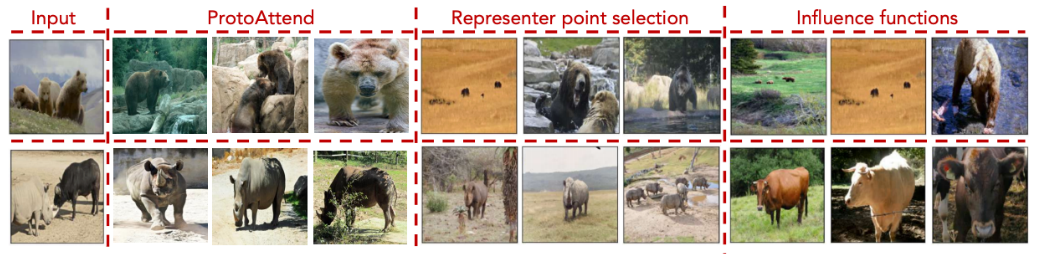
\includegraphics[width=\linewidth]{Arik2020.png}
  \caption{Samples found by ProtoAttend vs. representer point selection and influence function \cite{Arik2020}.}
\end{figure}

\begin{figure}
  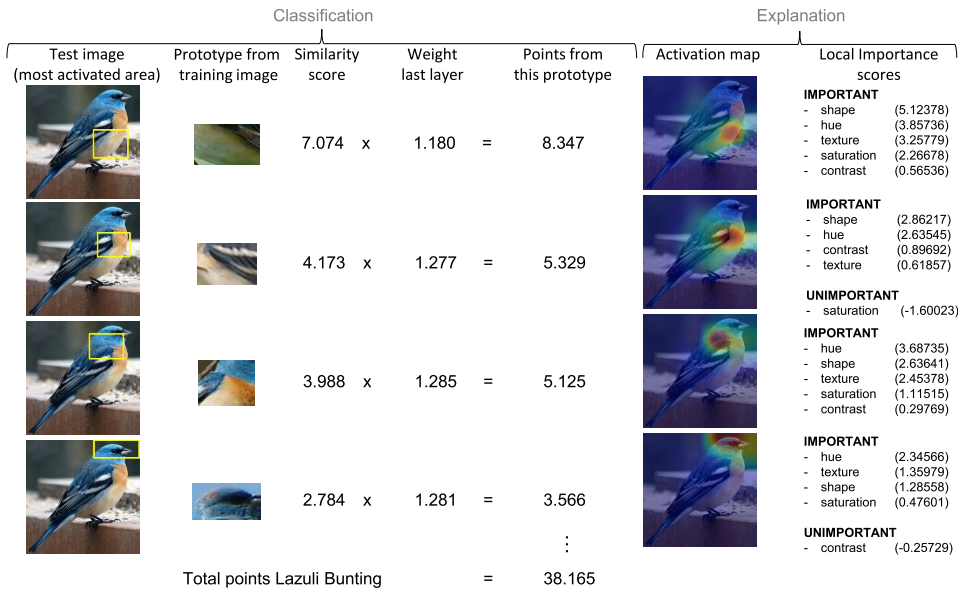
\includegraphics[width=\linewidth]{Nauta2020.png}
  \caption{ProtoPNet reasoning with a subset of all prototypes of the Lazuli Bunting class \cite{Nauta2020}.}
\end{figure}

\cite{Wei2017} proposes the use of influence functions to explain a model’s decision by tracing which instances from the training set were the more influential with respect to the input instance.
Similarly, \cite{Yeh2018} develops an explanation method that decomposes the prediction into a linear combination of activations of training points, termed as Representer Points. This method detects both positive and negative representative values corresponding to excitatory and inhibitory training points respectively.
ProtoAttend \cite{Arik2020} also employs this linear decomposition notion but the importance weights for the training instances are learned via an attention mechanism.
\cite{Caruana1999} provides the user with the entries of the training dataset that are the most similar to the to-be-explained instance, by appplying Euclidean metrics to all the input features.
In an analogous way, \cite{Haghighi2019} proposed to explain the recommendations of an autoencoder deep neural network based on the ratings of neighbouring users, i.e. users with similar preferences. 
\cite{Bien2011} formulates Prototype Selection (PS). This approach provides a global explanation in which every instance must have a prototype corresponding to its label in its neighborhood, no instances should have a prototype with a different label in its neighborhood, and there should be as few prototypes as possible.  
\cite{Kim2016} developed an algorithm called MMD-critic that analyzes a dataset to form prototype and critic groups corresponding to different instance classes.
\cite{Gurumoorthy2019} generalizes \cite{Kim2016} by building a framework that not only selects prototypes and criticisms but also associates importance weights to the instances composing each group. 
\cite{Li2018} introduced a novel architecture that bases its classification on prototypes which can concurrently be returned as explanations. The architecture consists of a multilayer convolutional autoencoder and a prototype classifier network. Firstly, the original image is fed into the encoder and the produced feature maps are flattened into a vector. Then, the distances betwen this and a set of prototype vectors (selected so to be representative of the whole training dataset) are computed and regarded as weights for a fully connected layer followed by a softmax layer that makes the classification. Additionally, the prototype vectors can be visualized via the decoder of the network to be returned as explanations of the resulted decision.
ProtoPNet (Prototypical Part Network) \cite{Chen2019} also followed this prototype layer approach. For all instances of the training dataset, the patches of the convolutional output that are the most relevant for identifying their class (i.e. the patches that cause the strongest activations) are selected. In this way, a set of prototype parts that represent each class is collected. Each input image is first passed through a number of convolutional layers. The resulting feature maps are fed to the prototype layer where the distances between all patches of these maps and each prototype part are computed. Based on these scores a fully connected layer makes the classification and the parts with the highest similarity can be returned as its interpretation.
\cite{Nauta2020} introduces an explainability method that can enhance any prototype similarity-based technique by providing extra information about visual characteristics that the model perceives as similar. Specifically, the similarity is justified based on the importance of color hue, shape, texture, contrast and saturation. To achieve this, the input image is perturbed with respect to each of these characteristics and the similarity measures between the prototype and the modified images are obtained. The importance of each visual trait can then be computed based on the difference between the prototype-image similarity of the original and the respectively perturbed images.
\cite{Angelov2020} developed another prototype-based explainable deep neural network architecture. The training of the introduced framework is carried out seperately for each class, as follows. Firstly, the feature layer (that can be formed by the fully connected layer of a pre-trained convolutional neural network) extracts feature vectors for each training image of the class. Based on these features, the density layer computes the proximity between the processed images. Then, these values are fed to the typicality layer that estimates a probability distribution function (pdf) of the images. The prototypes are extracted in the prototype layer as the peaks of this pdf. Finally, the neighbouring prototypes that belong to the same class are merged in the MegaClouds layer. Based on the prototype sets that are obtained during this training, the framework classifies a new unlabeled image in the following way. A feature layer, same as before, extracts feature vectors and the similarity between the input image and the nearest prototypes of each class is computed in the prototypes layer. Then, the prototype with the maximum similarity is selected per class in the next layer, the local decision-making layer, and, by obtaining the maximum of these similarities, the dominate class is determined in the global decision-making layer and the corresponding label is assigned to the input.

\subsubsection{Counterfactuals}
\hfill\\
The counterfactual approach indicates the minimum required alterations of the input features that would have led the network to an alternative decision \cite{Wachter2017}. The motivation behind this technique is that presenting users with a set of diversified examples can help shed light on how the system works, and can concurrently ease the adoption of these changes in case a different result is desirable \cite{Confalonieri2021}. 

\begin{figure}
  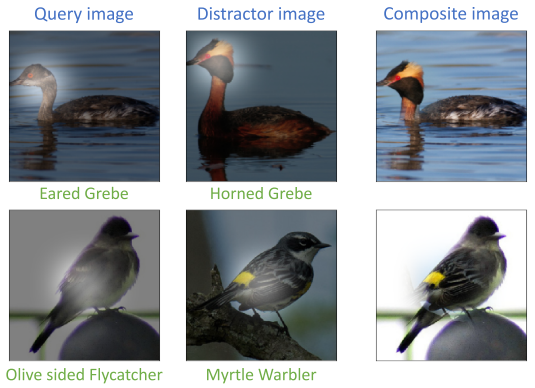
\includegraphics[width=\linewidth]{Goyal2019a.png}
  \caption{Counterfactual explanations \cite{Goyal2019a}.}
\end{figure}

\begin{figure}
  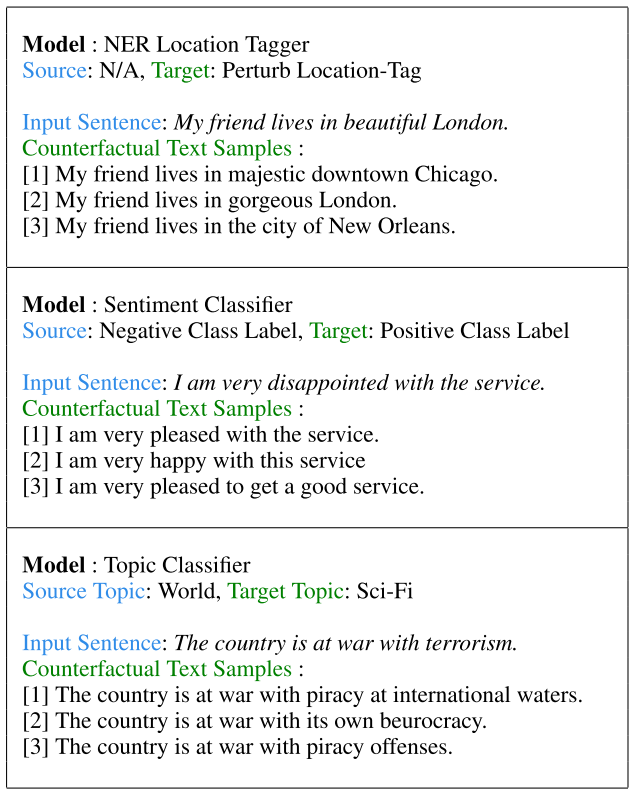
\includegraphics[width=\linewidth]{Madaan2020.png}
  \caption{Counterfactual samples generated by GYC \cite{Madaan2020}.}
\end{figure}

\cite{Mothilal2020} proposed DiCE (Diverse Counterfactual Explanations), a framework for providing counterfactual explanations based on determinantal point processes. The generated counterfactuals are optimized with respect to feasibility and diversity.
CERTIFAI (Counterfactual Explanations for Robustness, Transparency, Interpretability, and Fairness of Artificial Intelligence) \cite{Sharma2019} uses a custom genetic algorithm to generate counterfactuals that can explain any black-box model and any type of model data.
\cite{Ramon2019} introduces LIME-Counterfactual (LIME-C) and SHAP-Counterfactual (SHAP-C) by aligning the previously discussed methods LIME and SHAP with the notion of counterfactuals. Specifically, perturbations are utilized to find a set of features of the input instance (e.g. pixels or words) such that zeroing these features causes the predicted class to change. 
GYC (Generate Your Counterfactuals), developed in \cite{Madaan2020}, is an explanation framework that generates a set of counterfactual text samples for natural language processing (NLP) models. The generation of these counterfactuals can be directed towards a specified ‘condition’, such as the sentiment label, the topic or the location tag. 
\cite{Goyal2019a} implements counterfactual generation to explain image classification problems. Given the classification of an input image, this method selects another image that the model classifies differently and identifies special regions in the chosen image that replacing the corresponding regions in the input image would push its predicted class to be the same as the selected one. 
Also attending to the domain of image classification, CounteRGAN \cite{Nemirovsky2020} utilizes a Residual Generative Adversarial Network (RGAN) to generate realistic counterfactual explanations. 
\cite{Delaney2020} developed a counterfactual generation approach for time series classification tasks. More specifically, this method locates the nearest instance that belongs to a different class and uses it as a guide for altering the input time series to produce the desired counterfactual.
\cite{VanLooveren2019} similarly suggests a technique to utilize class representative prototypes to assist the counterfactual search procedure.
\cite{Vercheval2021} introduces VAEX, a Hierarchical VAE designed to to explain classifier networks by producing realistic counterfactuals, that reflect targeted modifications on selected semantic features of the original image whilst avoiding pixel loss.
\cite{Keane2020} proposes a methodology that leverages a set of 'good' counterfactual explanations, which are assumed to be already available or feasible, for the generation of other high-quality counterfactuals that can interpret new instances.
\cite{Downs2020} developed a novel recourse generating method, CRUDS (Counterfactual Recourse Using Disentangled Subspaces), that uses a Conditional Subspace Variational Autoencoder (CSVAE) to produce multiple paths that can alter a model's decision directed both by the data structure as well as the end-users.
CoCoX \cite{Akula2020} explains a CNN's decision by determining the semantic features, e.g. stripes or ears of a portrayed animal, that need to be introduced or ablated from an image to shift its prediction to another specified class.
\cite{Kanamori2020b} introduces DACE (Distribution-Aware Counterfactual Explanation), a method that generates counterfactual explanations taking into consideration the empirical data distribution.
\cite{Poyiadzi2020} developed FACE (Feasible and Actionable Counterfactual Explanations), an algorithm that considers density-weighted metrics to locate the shortest path distances and uses these optimal  “feasible paths” of change to generate counterfactual explanations.
\cite{Cheng2021} proposed DECE (Decision Explorer with Counterfactual Explanations), an interactive visual analytics tool that compute and present counterfactual explanations both on individual instances and data subsets. User interactions are also enabled to customize the generation process according to their individual needs.
ViCE (Visual Counterfactual Explanations) \cite{Gomez2020} is another interactive visualization interface that explains a model's decision by providing counterfactuals. The developed algorithm starts with a set of features whose alteration is plausible. Then, the values of each feature are altered to different directions and the directions that have the greatest effect on the output decision are selected. This procedure is repeated iteratively as long as the constraints allow it or until the model's decision changes.
\cite{OShaughnessy2020} proposed to construct counterfactual explanations based on the combination of a generative model that learns to represent the underlying data distribution and a causality-based method that selects the generated latent factors that are highly influencial to the classifier's decision. 
\cite{Mahajan2019} proposed a method that addresses the issue of counterfactual feasibility. The authors introduce a causal proximity regularizer based on constraints deducted by a structural causal model. For cases when constraints cannot be easily obtained, a VAE-based generative model is proposed that can learn to produce feasible counterfactuals based on user feedback.
\cite{Kanehira2019b} that generates counterfactual explanations for video classification tasks. Given spatio-temporal region and corresponding linguistic attributes, the proposed explanation model is trained to calculate [attribute, region] combinations that support the output class prediction against another class of interest.
Actionable Recourse Summaries (AReS) \cite{Rawal2020} generates a summary of counterfactual recourses for the entire training dataset of a model to globally explain it. Specifically, the framework learns rule sets that express the plausible recourses for subpopulations of the data and then aggregates them to obtain the desired summary.
\cite{Kanamori2020b} proposes a framework that calculates feasible counterfactual actions by evaluating their executability based on the empirical data distribution.
\cite{Kanamori2021} introduces Ordered Counterfactual Explanation (OrdCE), a framework that provides ordered counterfactual actions, by taking into consideration the order of the proposed feature perturbations. The optimal combination of actions and order are calculated based on feature interactions via a mixed-integer linear optimization objective.
\cite{Pollack2020} propose to gradually exaggerates features of the input instance to shift the posterior probability from the originally predicted class to its negation. Features that are irrelevant to the classification are preserved unaltered, so that the produced counterfactuals span across the data manifold in a way that clearly indicates the decision boundary of interest.
\cite{Kang2020} proposes an explanation method that gradually generates a counterfactual interpretation of the model's decision by iterating over masking and composition steps. The masking step locates the input features that are the most important to the output, and the composition step optimizes these features to set their output close to the logit space of the training data that belong to another target class. Hence, this method provides a combination of attribution and evidence based explanations.

\subsubsection{Concepts}
\hfill\\
High-level concepts, such as curls or strips, can also be presented as evidence to explain the prediction of a deep model.

\begin{figure}
  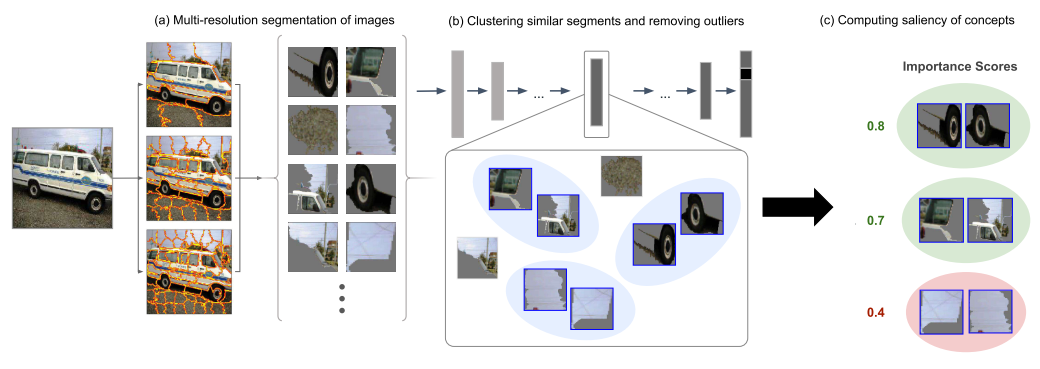
\includegraphics[width=\linewidth]{Ghorbani2019.png}
  \caption{ACE explanation procedure \cite{Ghorbani2019}.}
\end{figure}

\begin{figure}
  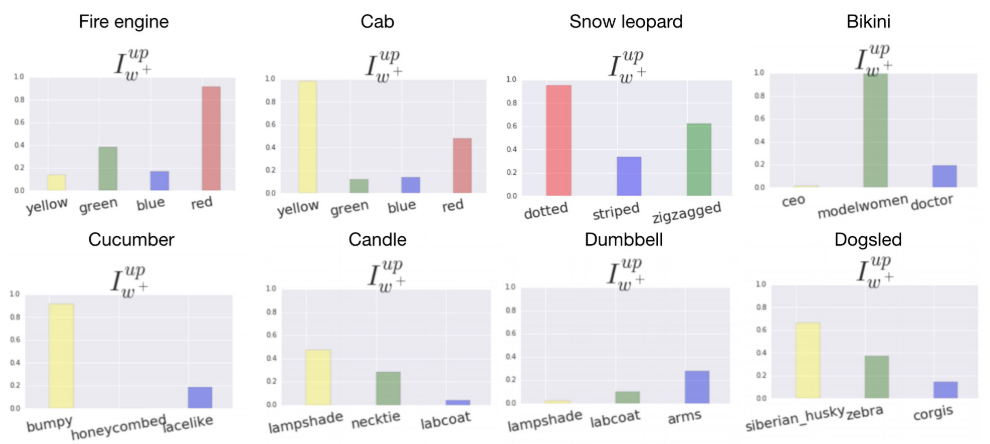
\includegraphics[width=\linewidth]{Kim2018a.png}
  \caption{Simplistic example of concept-based explanation generated by TCAV \cite{Kim2018a}.}
\end{figure}

\cite{Kim2018a} \cite{Kim2018} introduces Concept Activation Vectors (CAVs) and uses them in a novel method called Testing with CAVs (TCAV) that quantifies the degree to which a user-defined concept contributes to a classification prediction. Given input $x \in R^n$ and a feedforward layer $l$ having $m$ neurons, the activation at that layer is given by $f_l:R^n \to R^m$. Each class can be deduced to a set of positive concepts $P_C$, i.e. concepts that are humanly conceived as representative for this class (e.g. if a detected class is the animal zebra, then a positive concept would be stripes). A negative set of concepts $N$ can be gathered, for example a set of random photos, to contrast the concepts of the class. These two sets are used to train a binary classifier $v_C^l \in R^m$ that partitions ${f_l (x):x \in P_C}$ and ${f_l (x):x \in N}$. CAV is thus defined as the normal vector to the hyperplane that separates the positive examples from the negative ones. Then, directional derivatives are used to evaluate the sensitivity of class predictions of $f$ to the changes in given inputs towards the direction of a concept $C$ for a specific layer $l$. If $h(l,k)$ is the logit of layer $l$ for class $k$ for a particular input, the conceptual sensitivity of $k$ to $C$ can be computed as the directional derivative $S_{C,k,l}(x)=\nabla h_{l,k} (f_l (x)) \cdot v_C^l$ for a concept vector $v_c^l \in R^m$. A TCAV score can then be calculated to find the influence of inputs towards $C$: $TCAV_{Q_{C,k,l}}= \frac{|{x \in X_k:S_{C,k,l}(x)>0}|}{|X_k|}$, where $X_k$ denotes all inputs with label $k$. 
In \cite{Graziani2018} the authors extended TCAV, which originally considers the presence or absence of concepts, to detect continuous concepts. Instead of seeking a discriminator between two concepts, or one concept and random inputs, their method seeks the direction of greatest increase of the measures for a single continuous concept. Firstly, Regression Concept Vectors (RCVs) are computed via least squares linear regression of the concept measures for a set of inputs. Then, the relevance of the concept is measured with bidirectional relevance scores that assume positive or negative values based on how increasing values of the concept measures affect the classification.
A further improvement over the above two methods was introduced in \cite{Yeche2019} that used a new metric called Uniform unit Ball surface Sampling (UBS) to provide layer-agnostic explanations for continuous value concepts with improved scaling to high dimensional spaces. 
\cite{Ghorbani2019} developed a method called Automatic Concept-based Explanations (ACE) that improves on TCAV by being able to explain a trained classifier without human supervision. For a set of images from the same class, each image is segmented with multiple resolutions, e.g. texture, object parts and objects. All segments are resized to the standard input size of the model and outliers are removed. Then, the segments are clustered, as examples of the same concept, using the activation space of a specific chosen bottleneck layer as similarity space. Finally, TCAV scores are computed for each concept and the most important concepts are returned as an explanation for the particular classification. 
Causal Concept Effect (CaCE) \cite{Goyal2019} also improved the TCAV method by examining the causal effect of the retention or ablation of high level concepts towards a deep model’s prediction. In this way, the calculated concept measures are protected from the influence of biases or correlations in the dataset, which can fool methods like TCAV. CaCE can be computed exactly by using controlled environments that allow direct intervention on parts of the image generation process (GT-CaCE). Alternatively, a variational autoencoder (VAE) can be used to implement the interventions needed for the computation of CaCE (VAE-CaCE). 
\cite{Yeh2019} introduced ConceptSHAP, a method that employs the previously discussed SHAP method in presenting concepts that explain a model's prediction. Similar to ACE, ConceptSHAP uses segmentation and clustering to discover concepts from a dataset. However, ConceptSHAP computes the score of each individual concept by utilizing Shapley values for importance attribution. 
\cite{Godi2019} explains deep networks by providing 'visual summaries' of the detected classes. First, masks that highlight the most important regions of training images are computed, in a way similar to the perturbation-based attribution methods discussed previously. Then, the component regions of each class's masked instances are clustered together. In this way, every class can be represented by a set of visual concepts that interpret the parts that mainly led to the decision of the model.

\subsubsection{Description}
\hfill\\
Lastly, another form of explanatory evidence that can be provided to the end-user of a model are linguistic descriptions of the decision-making rationale. This is generally achieved by training an auxiliary model to produce these explanations based on captions or some other form of human generated interpretations.  

\begin{figure}
  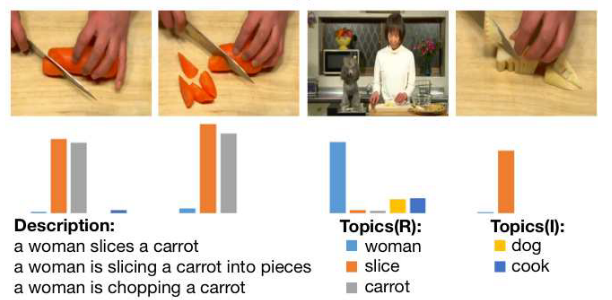
\includegraphics[width=\linewidth]{Dong2017.png}
  \caption{Activations of one neuron according to relevant (R) and irrelevant (I) topics through time in video action recognition \cite{Dong2017}.}
\end{figure}

\begin{figure}
  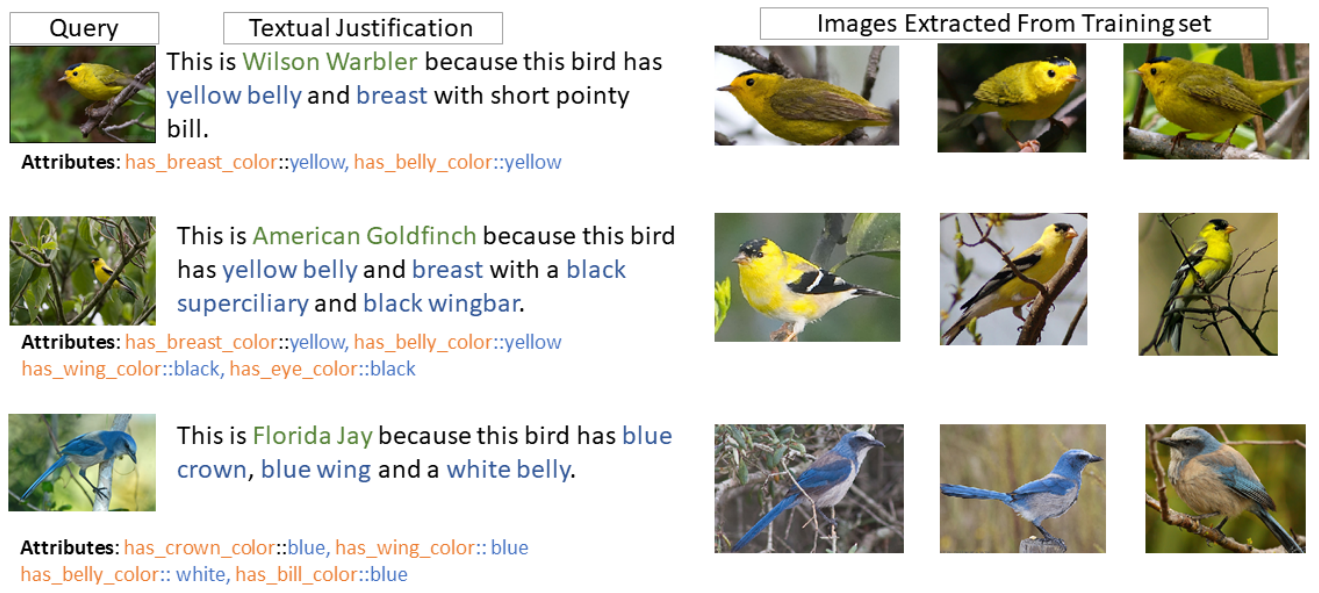
\includegraphics[width=\linewidth]{UlHassan2019.png}
  \caption{Visual explanation generated by EVCA \cite{UlHassan2019}.}
\end{figure}

\cite{Hendricks2016} introduced a method to justify image classification by providing natural language explanations. This is achieved by employing a caption method with a fine-grained recognition pipeline to produce strong features and then feeding the extracted captions to an LSTM that generates an explanatory sequence of words. A novel loss function, based on sampling and reinforcement learning, is suggested to optimize the sentence generation for class-specificity. 
\cite{Guo2018} proposed a method that aims to find a list of visual attributes that are the most important for a decision of the network. Firstly, image-level visual attributes for the training inputs are either obtained by decomposing image caption or through ground truth annotation. Then, the final convolutional layer filter is associated with these attributes, by calculating the filter attribute probability density function as a posterior probability, learned by a bayesian inference algorithm, with the input images as latent variables. Finally, based on the filter attribute probability density function (p.d.f.), the attributes are ranked by re-weighting each filter attribute p.d.f. with class specific weights. The top attributes are returned in a template sentence as evidence that explains the model's classification. 
\cite{Ehsan2018} \cite{Ehsan2019} established an AI rationalization technique, which treats the generation of explanations as a problem of translation between ad-hoc representations of states and actions in an autonomous system’s environment and natural language. To do this, first, a corpus of natural language utterances was collected from people that were asked to 'think aloud' while completing the agent task’s in a virtual environment. Then, this corpus was used along with state information to train an encoder-decoder neural network that translates between state-actions and natural language. This translation acts as a rationalization of the agent's behavior that can potentially be more satisfying than other types of explanations. 
EVCA (for Explaining Visual Classification using Attributes), developed in \cite{UlHassan2019}, uses captioning methods to generate descriptive attributes for each input image, a CNN for the classification task and then an LSTM to produce a natural language explanation that contains the classification class along with a list of attributes associated with the image. Additionally, it retrieves similar images from the training set, using pairwise distance and checking that they also contain the attributes. This means that EVCA provides a combination of evidence to justify the model's decision, both description and prototypes (discussed in a previous paragraph). 
\cite{Hind2019} introduced an explanation framework called TED (Teaching Explanations for Decisions). In addition to the usual two components that traditional ML models are trained on, a set of inputs $X$ and a corresponding set of labels/decisions/classifications $Y$, TED also requires a third component, an explanation $E$ for each decision. Based on this augmented training set, TED produces a classifier that predicts both labels and respective explanations. This is accomplished via a cartesian product approach that encodes $Y$ and $E$ together into a new classification $YE$, which, along with $X$, is provided to an ML algorithm to produce a classifier that predicts $YE$'s.
In a similar manner, GEF (Generative Explanation Framework) \cite{Liu2020}, a framework designed for NLP (Natural Language Processing) tasks, learns to produce explanations for its predictions by being fed fine-grained reasoning along with the training input and output pairs.
\cite{Wickramanayake2019} proposed FLEX (Faithful Linguistic Explanations), a method that explains a CNN's decision by returning both linguistic description and attribution maps. GradCAM (which was described in the attribution-based methods section) is utilized to obtain feature maps that are important for the model's prediction. Then, given caption word attributes of the images in the training dataset, FLEX introduces a novel way to associate words with features. For each noun/adjective $w$ in the caption dictionary, the method computes its co-occurence score with each feature $u$ as: $score(w,u)=\frac{2 \times occur(w,u)}{count(w)+count(u)}$, where $count(w)$ is the number of occurences of $w$ in the ground truth descriptions, $count(u)$ is the number of occurences of $u$ in the training dataset and $occur(w,u)$ is the number of times $u$ and $w$ occur together. The word $w$ is associated with the feature $u$ that has the highest score. Finally, based on the feature maps and the captions of the image dataset, as well as the word to feature assotiation, FLEX trains a model composed of two stacked LSTMs to generate linguistic justifications of the CNN's decisions.
\cite{Zhou2020} developed ELV (Explanations as Latent Variables), a framework that treats natural language explanations as latent variables that reflect the internal reasoning of a neural model. As opposed to previous akin methods, ELV requires only a small set of human annotated explanations for training. In the first step, called E-step, the generator $p(e|x,y)$ is trained to generate explanations given labeled data. For labeled data with annotated explanations the likelihood of the ground truth explanations is maximized. For labeled data without explanations the Kullback-Leibler (KL) divergence between the variational distribution $q_{\theta}(e|x,y)$ and the ground truth posterior $p(e|x,y)$, which is calculated with the help of the prediction model, is minimized. During the second step, called M-step, the explanations generated in E-step are used to train the predictor $p(y|x,e)$ with maximum likelihood estimation (MLE).
\cite{Kim2018b} develops an interpretable CADx (Computer Aided Diagnosis) framework (ICADx). During its training, the framework is fed with images of masses along with their corresponding standardized medical descriptions. Utilizing these inputs, a generative network is implemented to map the detected malignancies to radiologists' interpretations. A diagnostic CNN is trained jointly with this generator network to be able to provide explanatory descriptions along with its decisions.
\cite{Shen2019} introduces an HSCNN (Hierarchical Semantic Convolutional Neural Network) that is structured in a way that provides two levels of ouput;  low-level semantic features and a high-level prediction. The low-level module is composed of branches, each representing a distinct human comprehensive feature. These resulting features are utilized along with the input to compute the final high-level prediction, while at the same time operating as interpretation of this decision.
Given a set of descriptive attributes corresponding to each class as input, \cite{Gulshad2020} proposes to learn a function that maps training images close to their respective class properties. Then, to interpret a prediction, the input instance is perturbed and attributions are predicted for both the clean and the adversial image via the computed mapping function. Based on the similarity between these two sets of attributes, the properties that are mostly important for the prediction are selected and provided as explanations. Directed perturbations are also applied to classify the image into a different class and observe the effect on its attributions. In this way, the method can additionally provide 'counter-attributes' and 'counter-examples' as explanations, resembling the previously discussed counterfactual technique.
InterpNET \cite{Barratt2017} also utilizes a dataset that contains classified images along with respective class-discriminative descriptions. A large set of features is extracted for each image via a bilinear compact pooling network and fed to a fully connected (FC) network that classifies the image. The internal activations of the FC network are then provided as inputs to an RNN trained on the aforementioned dataset to generate a linguistic explanation of the classification.
\cite{Kanehira2019a} introduces a framework that equips a CNN predictor with two interpretation modules; the explainer and the selector. The explainer generates a vector containing attribute values that describe the input image, based on explanations that were included in the training dataset. The selector uses the input and the produced linguistic explanation to select a few example instances that are most similar to the prediction of interest. 

\section{Network explanation}
Network explanation concerns the explanation of the distribution of knowledge that is formed inside the model, for example which layers have learned to represent each class, or how the learning evolves during the training epochs. This class of methods tends to focus on several different objectives that are discriminated followingly. 

\subsubsection{Preferred input}
\hfill\\
A common objective is visualizing the preferred inputs of neurons in each layer to indicate what features they have learned. 

\begin{figure}[h!]
  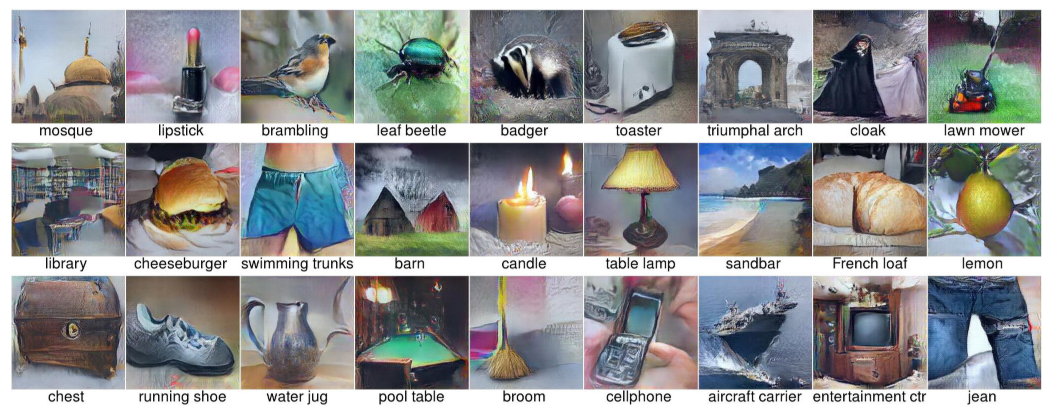
\includegraphics[width=\linewidth]{Nguyen2016.png}
  \caption{Images synthesized from scratch to highly activate certain output neurons \cite{Nguyen2016}.}
\end{figure}

\begin{figure}[h!]
  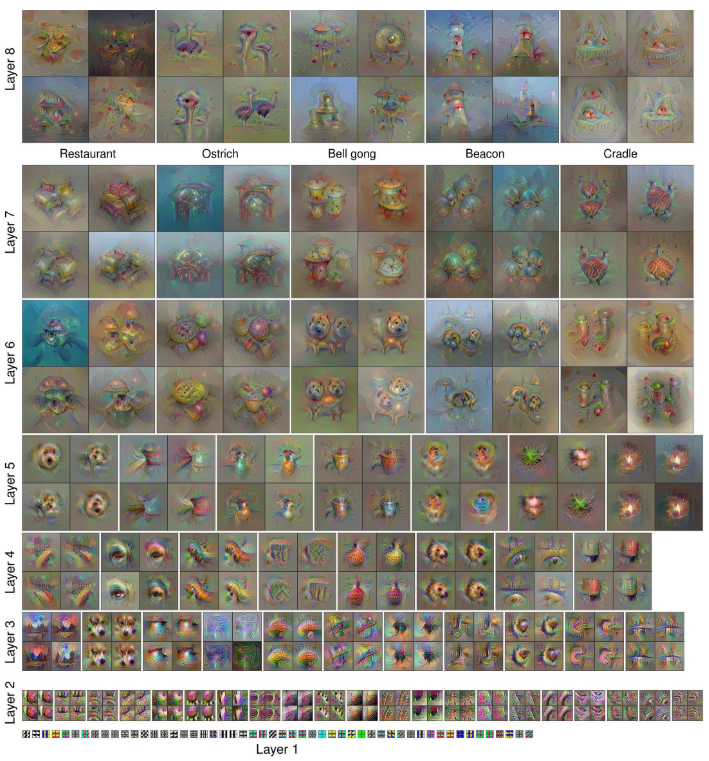
\includegraphics[width=\linewidth]{Nguyen2016a.png}
  \caption{Multifaceted visualization of example neuron feature detectors from all eight layers of a deep convolutional neural network \cite{Nguyen2016a}.}
\end{figure}

The fundamental algorithm, termed as Activation Maximization (AM), was introduced in \cite{Erhan2009} \cite{Erhan2010} that proposed to visualize important features in any layer of a deep architecture by synthesizing an image $x^*$ which maximizes the activation $a$ of the chosen unit $i$ in a layer $l$: $x^*=argmax_x a_{i,l} (\theta,x)$, where $\theta$ denotes the fixed network parameter sets (weight and bias). Firstly, an image $x=x_0$ with random pixel values is set to be the input to the activation computation. Next, the gradients with respect to the noise image $\frac{\partial{a_{i,l}}}{\partial{x}}$ are computed using backpropagation. Then, each pixel of the noise image is changed iteratively to maximize the activation of the neuron, by applying the update: $x \gets x+\eta \cdot \frac{\partial{a_{i,l}(\theta,x)}}{\partial{x}}$ where $\eta$ denotes the gradient ascent step size. This process terminates on convergence, returning a specific pattern $x^*$ that is considered the preferred input for the target neuron.  
\cite{Nguyen2016} built on the original activation maximization technique by utilizing an image generator network for the pixel tuning. This results in a more realistic synthesized image, which greatly improves the interpretability of the visualized patterns. This method is called Deep Generative Network Activation Maximization (DGN-AM). The DGN-AM implementation can be viewed as: $x^*=argmax_x (a_{i,l}(\theta,G(x))-\lambda(x))$, where $G$ indicates the generative network that takes the initial noise image as input.
The above activation maximization techniques generate images without taking into consideration that each neuron can fire in response to different types of related features (e.g. the bell pepper class detects bell peppers of different colors, alone or in groups, cut open or whole, etc.), thus creating inappropriate mixes of colors, parts of objects, scales, orientations, etc. To tackle this, \cite{Nguyen2016a} proposed MFV (Multifaceted Feature Visualization), a method that separately synthesizes the multiple facets of each neuron by introducing an alternative initialization procedure for the activation maximization algorithm. To obtain an initialization per facet, the training images that maximally activate a neuron are projected into a low dimensional space and then clustered via k-means, and finally the n closest images to each cluster centroid are averaged to produce the initial image. The authors also introduced a novel center-biased regularization technique which reduces AM’s tendency to produce repeated object fragments and instead tends to produce one central object. This is achieved by allowing more optimization iterations for center pixels than edge pixels.
\cite{Nguyen2017} improves the diversity and quality of the samples produced via DGN-AM \cite{Nguyen2016} by introducing an additional prior that directs optimization to realistic-looking images. This is done by developing a probabilistic framework for activation maximization based on a novel type of energy-based models, called Plug and Play Generative Networks (PPGN), where the energy function is a sum of multiple constraint terms: (a) priors, that can for example bias images to look realistic, and (b) conditions, that are typically a category of a separately trained classification model. An approximate Metropolis-adjusted Langevin algorithm is used to sample iteratively from these models. In essence, PPGNs are composed of a generator network capable of drawing a wide range of image types and a replaceable “condition” network that directs what the generator produces. Hence, one is free to design an energy function, and “plug and play” with different priors and conditions to form a new generative model. Moreover, instead of conditioning on a class output neuron, PPGNs can condition on a hidden neuron, revealing many facets that a neuron has learned to detect. Thus, this method can also be seen to improve the aforementioned MFV \cite{Nguyen2016a} which generates the set of synthetic inputs that activate a neuron to gain a better understanding of its stimulus preferencies.

\subsubsection{Concept distribution}
\hfill\\
Another form of network explanation seeks to shed light on the way various semantic concepts (i.e. humanly conceived entities or properties, such as man, chair, stripes, color) are represented throughout a trained network.

\begin{figure}
  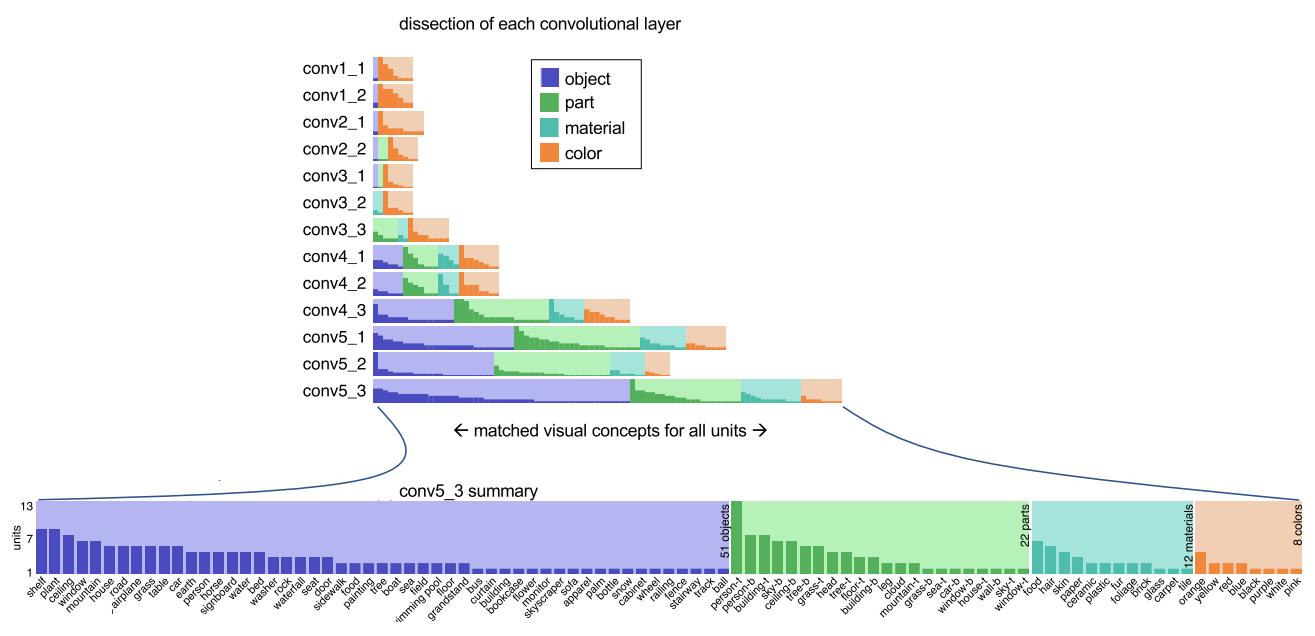
\includegraphics[width=\linewidth]{Bau2020.png}
  \caption{Dissection of a CNN object detector \cite{Bau2020}.}
\end{figure}

\begin{figure}
  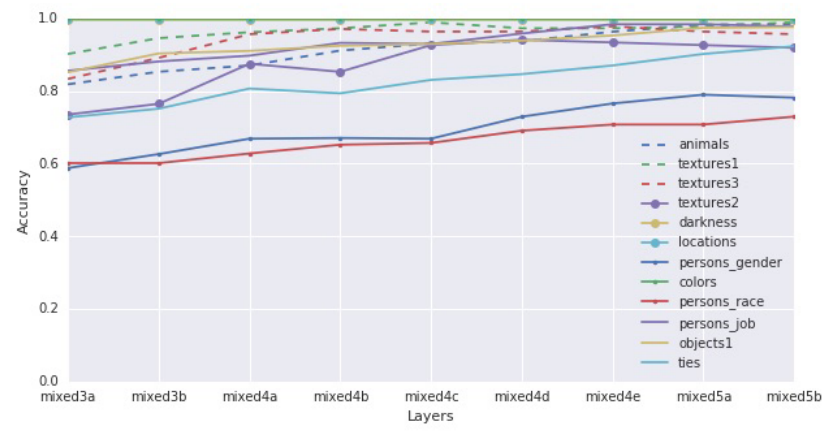
\includegraphics[width=\linewidth]{Kim2018a_b.png}
  \caption{Where each of the CAVs are learned \cite{Kim2018a}.}
\end{figure}

\begin{figure}
  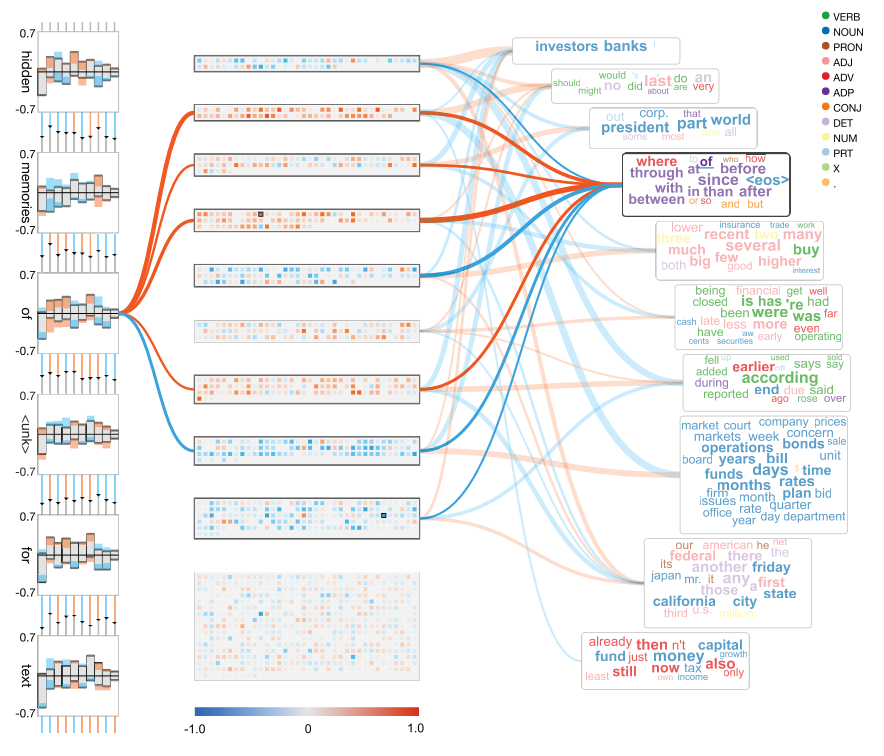
\includegraphics[width=\linewidth]{Ming2018.png}
  \caption{Glyph-based sentence visualization, memory chips visualization for hidden state clusters, and word clouds visualization for word clusters (left to right) \cite{Ming2018}.}
\end{figure}

Network Dissection \cite{Bau2017} \cite{Zhou2019} \cite{Bau2020} associates each convolutional neuron with semantic concepts of six kinds; scene, object, part, material, texture, and color. The authors unified several densely labeled image datasets to create the Broden dataset (Broadly and Densely Labeled Dataset) that provides a ground truth set of exemplars for a set of visual concepts. In addition, masks were applied to cover the image content not related to the assigned semantics. The correlation of a convolutional neuron, or multiple neurons, with each concept was evaluated by locating the neurons that strongly respond to image content with the specific semantic concept. This analysis allows the examination of what concepts and concept categories (color, object, part, material) are represented in each layer, which can shed light into how the network conceives information.
Net2Vec \cite{Fong2018} likewise maps semantic concepts to corresponding individual DNN filter responses, in a way very similar to Network Dissection. 
GAN Dissection \cite{Bau2018} was designed to understand the inferential process of GANs (Generative Adversarial Networks) at different levels of abstraction (unit-, object- and scene-level). Firstly, images generated by the network are segmented and the correlation of individual units’ feature maps to image regions is calculated. The units with the highest correlations are ablated by zeroing their activations and the average causal effect of this ablation is examined. In this way, the method uncovers semantic concepts that units (or groups of units) are related to. 
\cite{Ming2018} introduced a method to explain the concept distribution inside recurrent neural networks (RNNs), as well as two of their variants; long short-term memory (LSTM) networks and gated recurrent units (GRUs). More specifically, the authors proposed a technique to measure the response of hidden state units to input words. Based on these responses hidden units are clusterred to `memory chips' and words to `word clouds' (which can be considered as concepts), and a bipartite graph that associates the two is constructed. Part Of Speech (POS) tags are utilized as well to further illuminate the hidden units' functionality. Furthermore, the authors described a glyph-based technique to extend the method to sentence-level associations by aggregate information.
\cite{Dong2017} proposes a method that computes the association between neurons and topics on the video captioning domain. Using the human descriptions that compose the training dataset, a semantically wide set of 'meaningful topics' are extracted. Then, the desired neuron-concept correspondence is estimated by computing the effect of the ablation of each individual neuron with respect to each topic for all the videos in the traning set.
The previously discussed method TCAV \cite{Kim2018a} \cite{Kim2018} can also be utilized to explain where each concept is learned in the network by examining the accuracy of the linear classifiers at every layer for each type of CAV.

\subsubsection{Class distribution}
\hfill\\
Several methods have also been developed to clarify how knowledge about the target classes is distributed across the neurons or layers of a deep neural network.

\begin{figure}
  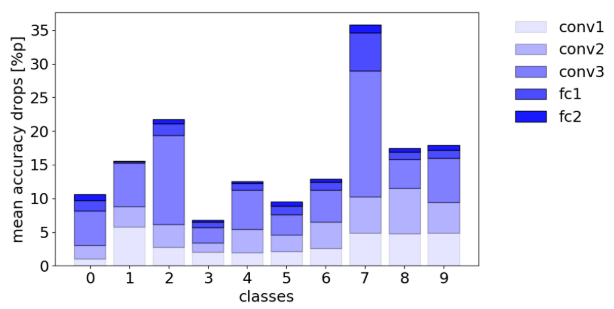
\includegraphics[width=\linewidth]{Meyes2020.png}
  \caption{Stacked bar plot of mean accuracy changes as a result of network ablations \cite{Meyes2020}.}
\end{figure}

\begin{figure}
  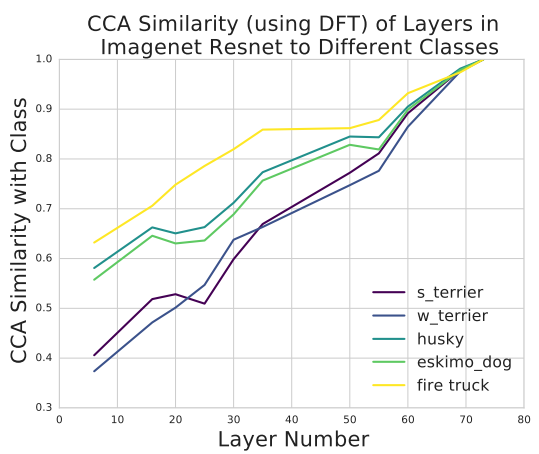
\includegraphics[width=\linewidth]{Raghu2017.png}
  \caption{CCA similarity using the Discrete Fourier Transform between the logits of five classes and layers \cite{Raghu2017}.}
\end{figure}

SVCCA (singular vector canonical correlation analysis) \cite{Raghu2017} is a network explainability method that combines CCA (Canonical Correlation Analysis) and SVD (Singular Value Decomposition). SVCCA finds out the relation between two layers of a network $l_k=(z_1^{l_k},…,z_{m_k}^{l_k})$ for $k = 1,2$, where $z_i^l=(z_i^l (x_1 ),…,z_i^l (x_m ))$ is the activation of neuron $i$ at layer $l$ given an input data set $X=\{x_1,…,x_m\}$. SVCCA uses SVD to extract the most informative components $l_k'$ and uses CCA to transform $l_1'$ and $l_2'$ so that $\bar{l_1}=W_X l_1'$ and $\bar{l_2}=W_Y l_2'$ have the maximum correlations $\rho=\{\rho_1,…,\rho_{min(m_1',m_2')}\}$. The algorithm returns the aligned directions $(\bar{x_i},\bar{y_i})$ and how well they align $\rho_i$, along with the singular values and directions $\lambda_X^{(i)}$, $x'^{(i)}$, $\lambda_Y^{(j)}$, $y'^{(j)}$. In this way, SVCCA can be used to measure the class distribution throughout the network by comparing the correlation of representations in each layer with the logits of each class. SVCCA can also illuminate how the representation at each layer evolves during training, by comparing the final instance of the given DNN to other instances of the network at different points in the training process.
\cite{Meyes2020} iteratively ablates half of the units within each layer and measures the drop in accuracy for all classes. Based on these ablation effects, the capacity that every layer devotes to the representation of each class can be computed and visualized to reveal the respective distributions.
To promote class-filter interpretability, \cite{Liang2020} proposes a strategy for training CNNs in a way that encourages class-specific filter formulation. Specifically, a novel structure called Class-Specific Gate (CSG) is introduced in addition to the standard (STD) path of forward propagation. CSG allows a filter's activation to pass only when the input samples come from a specific assigned class. In this way, the CSG path acts as regularization for filter differentiation training. 

\subsubsection{Information plane}
\hfill\\
Lastly, there is a family of methods that promotes the understanding of a DNN's inner workings by analyzing its information plane; the plane of the mutual information between the input and output variables.

\begin{figure}
  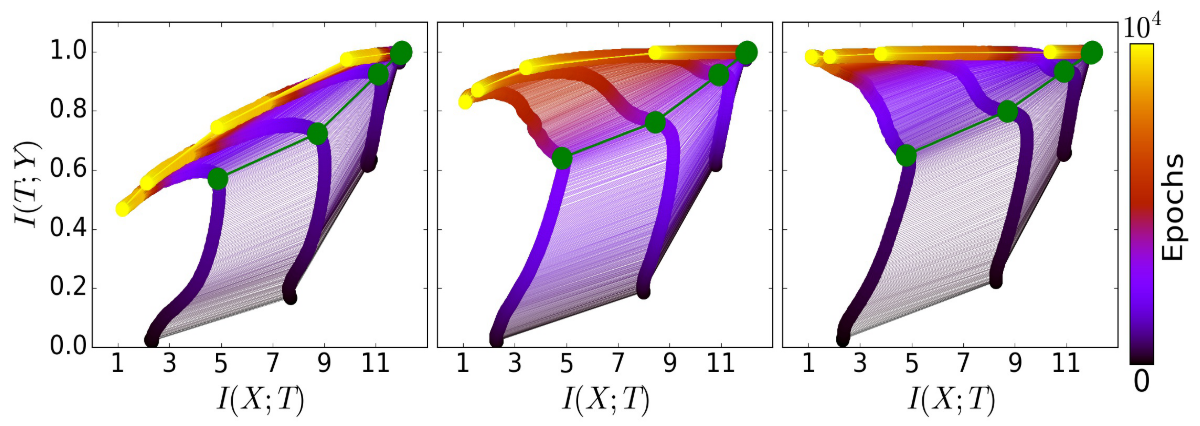
\includegraphics[width=\linewidth]{Shwartz-Ziv2017_b.png}
  \caption{The evolution of the layers with the training epochs in the information plane, for different training samples (5\%,  45\% and 85\% of the data, left to right) \cite{Shwartz-Ziv2017}.}
\end{figure}

This notion was seminally proposed in \cite{Tishby2000} as the Information Bottleneck (IB) method, which describes the problem of representing an observation $X$ in a lossy manner, such that its representation $T$ is informative of a relevance variable $Y$. Mathematically, the IB problem aims to find a lossy compression scheme described by a conditional distribution $P_{T|X}$ that is a minimizer of the following functional: $min_{P_{T|X}}(I(X;T)-\beta I(Y;T))$.
In \cite{Tishby2015}, it was proposed to analyze deep neural networks via the IB framework prinicple, by showing that any DNN can be quantified by the mutual information between the layers and the input and output variables. This representation promotes the calculation of the optimal information theoretic limits of the DNN, leading to the attainment of finite sample generalization bounds and the simplification of the network. It was also suggested that the goal of the network is to optimize the tradeoff between compression and prediction, successively for each layer.
\cite{Shwartz-Ziv2017} continued to build on this idea by demonstrating several points of understanding that the Information-Plane visualization offers about DNNs. Specifically, it was shown that there are two distinct phases in the course of deep learning training; in the first the layers increase the information on the labels (fitting) and in the second the layers reduce the information on the input (compression). The second phase is proven to be much longer and it amounts to a stochastic relaxation that maximizes the conditional entropy of the layers subject to the empirical error constraint. Furthermore, it was demonstrated that the maps from the input to each layer (encoder) and from the layer to the output (decoder) satisfy the IB self-consistent optimality conditions. Lastly, it was established that the main advantage of hidden layers is training acceleration as they reduce the stochastic relaxation times. This slowing down of the relaxation process near phase transitions on the IB curve causes the hidden layers to converge to such critical points.
\cite{Alemi2017} proposed Deep Variational Information Bottleneck (Deep VIB), a variational approximation of \cite{Tishby2000} that allows the compression scheme $P_{T|X}$ and the conditional distribution $P_{Y|T}$ to be parameterized by NNs, as well as the use of the reparameterization trick to enhance training efficiency.
\cite{Kolchinsky2019} parameterizes the information bottleneck model via neural networks trained to minimize an upper bound on $(I(X;T))^2-\beta I(Y;T)$ using a combination of variational and non-parametric bounding approaches. 
\cite{Fischer2020} formulates the principle of minimum necessary information and derives from it the conditional entropy bottleneck functional, which uses the chain rule of mutual information to replace $I(X;T)$ by $I(X;T|Y)$. 
\cite{Li2021} employed the IB theory to understand the inner behavior of convolutional neural networks. Interestingly, it was demonstrated that the compression phase is not observed in some cases, suggesting, in contrast to the conclusions of \cite{Shwartz-Ziv2017}, that compression is not a universal mechanism in deep learning.

\section{Conclusion}
Explainable deep neural networks is an open and active field of research, with various approaches emerging every year. This paper presents a clear categorization and comprehensive overview of existing explainability techniques, aiming to provide a good insight into the current progress on xDNNs and a deeper understanding of their application. Considerable research has been focused on post-model explainability algorithms due to the ease of their application. Furthermore, the great majority of the developed methods aim to explain the models’ predictions. Therefore, it seems that more focus is needed towards approaches that shed light into the inner behavior of the networks, in order to promote a more holistic advancement of the domain. 


\ifCLASSOPTIONcaptionsoff
  \newpage
\fi


\printbibliography


\vfill


\end{document}


